\documentclass[prb,11pt,tightenlines,twocolumn,aps]{revtex4-1}

\usepackage{amsmath}    % need for subequations
\usepackage{graphicx}   % need for figures
\usepackage{verbatim}   % useful for program listings
\usepackage{color}      % use if color is used in text
\usepackage{subfigure}  % use for side-by-side figures
\usepackage{hyperref}   % use for hypertext links, including those to external
                        % documents and URLs 
\usepackage{blindtext}  % fill text
\usepackage[dvipsnames]{xcolor}
\usepackage{multirow}
\usepackage[capitalize]{cleveref}
% \usepackage{showframe}
\usepackage[inline]{showlabels}

\raggedbottom           % don't add extra vertical space

\begin{document}

\title{Pure Spin Current Injection in Hydrogenated Graphene Structures}
\author{Reinaldo Zapata-Pe\~na\textsuperscript{1},
        Bernardo S. Mendoza\textsuperscript{1},
        Anatoli I. Shkrebtii\textsuperscript{2}}
\affiliation{\textsuperscript{1}Centro de Investigaciones en \'Optica, Le\'on,
Guanajuato 37150, M\'exico}
\affiliation{\textsuperscript{2}University of Ontario, Institute of Technology,
Oshawa, ON, L1H 7L7, Canada}

\date{\today}

\begin{abstract}
\blindtext
\end{abstract}

\maketitle

%%%%%%%%%%%%%%%%%%%%%%%%%%%%%%%%%%%%%%%%%%%%%%%%%%%%%%%%%%%%%%%%%%%%%%%%%%%%%%
%%%%%%%%%%%%%%%%%%%%%%%%%%%%%%%%%%%%%%%%%%%%%%%%%%%%%%%%%%%%%%%%%%%%%%%%%%%%%%
%%%%%%%%%%%%%%%%%%%%%%%%%%                         %%%%%%%%%%%%%%%%%%%%%%%%%%%
%%%%%%%%%%%%%%%%%%%%%%%%%% I N T R O D U C T I O N %%%%%%%%%%%%%%%%%%%%%%%%%%%
%%%%%%%%%%%%%%%%%%%%%%%%%%                         %%%%%%%%%%%%%%%%%%%%%%%%%%%
%%%%%%%%%%%%%%%%%%%%%%%%%%%%%%%%%%%%%%%%%%%%%%%%%%%%%%%%%%%%%%%%%%%%%%%%%%%%%%
%%%%%%%%%%%%%%%%%%%%%%%%%%%%%%%%%%%%%%%%%%%%%%%%%%%%%%%%%%%%%%%%%%%%%%%%%%%%%%

\section{Introduction}
\label{sec:introduction}


\begin{figure}[ht!]
    \centering
    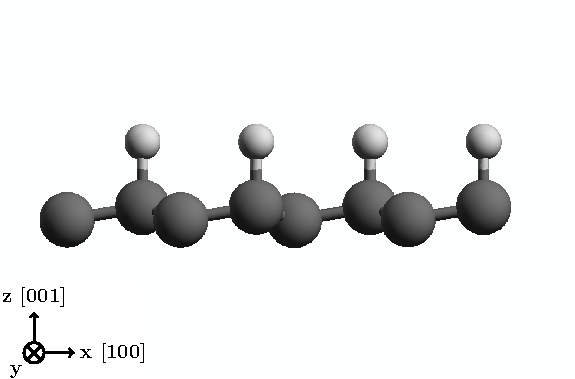
\includegraphics[width=\linewidth]{figures/upstruc2}
    \\
    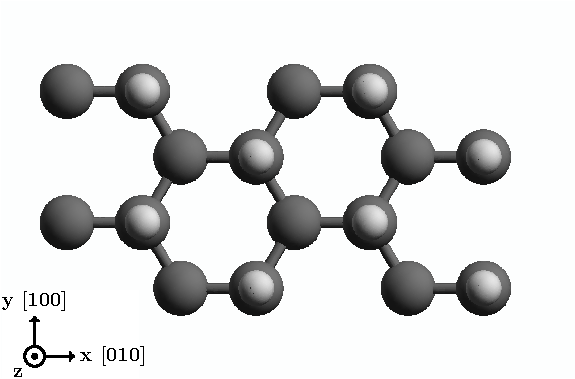
\includegraphics[width=\linewidth]{figures/upstruc1}
    \caption{Up structure}
    \label{fig:up-struc}
\end{figure}
\begin{figure}[ht!]
    \centering
    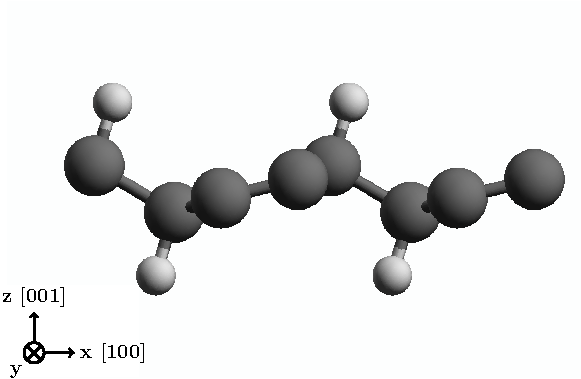
\includegraphics[width=\linewidth]{figures/altstruc2}
    \\
    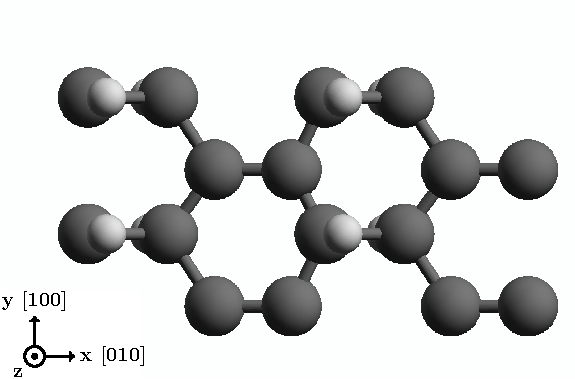
\includegraphics[width=\linewidth]{figures/altstruc1}
    \caption{Alt structure.}
    \label{fig:alt-struc}
\end{figure}


Spintronics is an emerging research field of electronics in which the
manipulation and transport of spin of electrons in a solid state 
media plays the determining role adding a new degree of freedom to the
conventional charge manipulation.\cite{wolfSC04,fabianAPS07}
% 
At present there is an increasing interest in attain the same level of control
over the transport of spin at micro or nano scales as has been done for the
flow of charge in typical electronic devices.\cite{awschalomNP2007} Some
semiconductor spintronics devices have been proposed \cite{majumdarAPL06,
dattaAPL90,gotteNat16,pershinPRB08} and some of them require spin polarized
electrical current \cite{awschalomSSBM13} or pure spin current (PSC).
% 
One of the difficulties to achieve the development of spin current and PSC
semiconductor devices is the fact that the spin relaxation time in a
semiconducting media is short disabling the spin transport and then resulting
in a no observable spin current.\cite{murakamiSc03}
% 
In PSCs there is no net
motion of charge; spin-up electrons move in a given direction while spin-down
electrons travel in the opposite one. This phenomena can result from spin
injection,\cite{malPRB03} Hall Effects,\cite{sinovaPRB04} interference of two
optical beams,\cite{bhatPRL00, najmaiePRB03} or one photon absorption of
linearly polarized light\cite{bhatPRL05} and has been observed in gallium
arsenide (GaAs),\cite{zhaoPRL2006, stevensPRL03} aluminum-gallium arsenide
(AlGaAs),\cite{stevensPRL03} and Co$_2$FeSi.\cite{kimuraNGPAM12}

Graphene, an allotrope of carbon with hexagonal 2D lattice structure presents
properties like fractional quantum Hall effect at room temperature, excellent
thermal transport properties, excellent conductivity\cite{heerscheNat07} and
strength \cite{geimNM07, reinaNL08, novoselov2S07, balandinNL08} being then a
perfect platform to be used in two-dimensions electronic systems; however most
electronic applications are disabled by the absence of a semiconducting gap.
Recent studies demonstrate that the band gap of graphene can be opened by
applying an electric field,\cite{zhangN09} reducing the surface
area,\cite{hanPRL07} or applying uniaxial strain.\cite{niACSN08} Another
possibility to open the gap is by doping; this has been successfully achieved
using nitrogen,\cite{weiNL2009} boron-nitrogen,\cite{guoIJ11}
silicon,\cite{colettiPRB10} noble-metals,\cite{varykhalovPRB10} and
hydrogen.\cite{eliasS09, guisingerNL09, samarakoonACSN10}
% 
Depending on the percentage of hydrogenation and spatial configurations of
hydrogen-carbon bonds, hydrogenated graphene can result in different spatial
configurations.
% 
In this paper we present two 50\% hydrogenated graphene noncentrosymmetric
structures both presenting a discernible band gap: the \emph{up} structure,
shown in Fig. \ref{fig:up-struc}, has hydrogen atoms bonded to the carbon layer
only in the upper side of the structure while the \emph{alt} structure, shown
in Fig. \ref{fig:alt-struc}, has hydrogen alternating in the upper and bottom
sides of the carbon slab.\cite{zapataPSB2016}

Using those structures we address a theoretical study of the spin velocity
injection (SVI) by one-photon absorption of linearly polarized light.
% 
% We calculated the responses for the particular cases when the spin of
% electrons is directed along the the $z$ Cartesian coordinate, perpendicular
% to the $xy$ plane of the structure, or for the case when the velocity is
% directed along the $x$ and $y$ Cartesian direction on the $xy$ plane of the
% structures.
{\color{red}
% 
Because we have 2D structures we made the analysis for tow cases. The first is
fixing the spin of the electrons along the $z$ Cartesian direction with the
velocity directed on the surface of the structure in the $xy$ plane. The second
is fixing the spin velocity in the $x$ or $y$ direction and the spin directed
in $xyz$.}
% 
The SVI is an optical effect that quantifies the velocity at which a PSC moves
along the Cartesian direction $\mathrm{a}$ with the spin of electron polarized
along the Cartesian direction $\mathrm{b}$. One photon absorption of linearly
polarized light can promote a distribution of electrons in $\mathbf{k}$ space
regardless the symmetry of the material resulting in a null electrical current.
Then, the electrons excited to the conduction bands at opposite $\mathbf{k}$
points will result in opposite spin polarizations producing no net spin
injection.\cite{bhatPRL05} If the crystalline structure of the material is
noncentrosymmetric the spin polarization injected at a given $\mathbf{k}$ point
could not vanish\cite{alvaradoPRL85, schmiedeskampPRL88} 
% 
{\color{red}
% 
and then, since the velocities of electrons at opposite $\mathbf{k}$ points are
opposite, a pure spin current will be produced. Since the structures presented
here are noncentrosymmetric, they are good candidates in which this effect can
be induced.}

This paper is organized as follows. In Section \ref{sec:theory} we present the
theory and formulas that describe PSC and SVI. In Section \ref{sec:results} we
describe the details of calculations and the corresponding SVI spectra for the
\emph{up} and \emph{alt} structures. Finally, we present our conclusions in
Section \ref{sec:conclusions}.


%%%%%%%%%%%%%%%%%%%%%%%%%%%%%%%%%%%%%%%%%%%%%%%%%%%%%%%%%%%%%%%%%%%%%%%%%%%%%%
%%%%%%%%%%%%%%%%%%%%%%%%%%%%%%%%%%%%%%%%%%%%%%%%%%%%%%%%%%%%%%%%%%%%%%%%%%%%%%
%%%%%%%%%%%%%%%%%%%%%%%%%%%%%%%%               %%%%%%%%%%%%%%%%%%%%%%%%%%%%%%%
%%%%%%%%%%%%%%%%%%%%%%%%%%%%%%%%  T H E O R Y  %%%%%%%%%%%%%%%%%%%%%%%%%%%%%%%
%%%%%%%%%%%%%%%%%%%%%%%%%%%%%%%%               %%%%%%%%%%%%%%%%%%%%%%%%%%%%%%%
%%%%%%%%%%%%%%%%%%%%%%%%%%%%%%%%%%%%%%%%%%%%%%%%%%%%%%%%%%%%%%%%%%%%%%%%%%%%%%
%%%%%%%%%%%%%%%%%%%%%%%%%%%%%%%%%%%%%%%%%%%%%%%%%%%%%%%%%%%%%%%%%%%%%%%%%%%%%%

\section{Theory} % (fold)
\label{sec:theory}


%%%%%%%%%%%%%%%%%%%%%%%%%%%%%%%%%%%%%%%%%%%%%%%%%%%%%%%%%%%%%%%%%%%%%%%%%%%%%%
%%%%%%%%%%%%%%%%%%%%%%%%%%% Theory: Spin velocity %%%%%%%%%%%%%%%%%%%%%%%%%%%%
%%%%%%%%%%%%%%%%%%%%%%%%%%%%%%%%%%%%%%%%%%%%%%%%%%%%%%%%%%%%%%%%%%%%%%%%%%%%%%


In this section, we report a summary of the theory that involves the PSC
phenomena from which rises the SVI treated in this paper.
 
In PSCs there is no net motion of electrical charge and spin-up electrons move
in a given direction while spin-down electrons travel in the opposite one.
This effect can result from one photon absorption of linearly polarized light
by a semiconductor, with filled valence bands and empty conduction bands,
illuminated by light with photon energy larger than the energy gap.
% note 1
Using a single continuous linearly polarized laser beam, it is possible
to promote electrons in $\mathbf{k}$ space regardless the symmetry of the
system resulting in a net current equal to zero. 
% 
If the phenomena is produced in a noncentrosymmetric semiconducting media, the
electrons promoted to the conduction bands at opposite $\mathbf{k}$ points
can produce a net spin polarization different to zero\cite{alvaradoPRL85},
resulting in a PSC because the velocity of electrons
at opposite $\mathbf{k}$ points are in opposite directions.

Using the multiple scale approach to solve the equation of motion for the
single particle density matrix $\rho_{mn}(\mathbf{k};t)$ we have that 
\begin{equation*}
\begin{aligned}
&\frac{\partial \rho_{cc'}}{\partial t} =
-i (\omega_{cc'} - i \epsilon) \rho_{cc'}
+
\frac{e^{2}E^{\mathrm{a}}(\omega)E^{\mathrm{b*}}(\omega)}
{i \hbar^{2}}
\times \\
& \quad \sum_{v}r^{\mathrm{a}}_{cv} r^{\mathrm{b}}_{vc'}
\left( \frac{1}{\omega - \omega_{c'v} - i \epsilon} 
- 
\frac{1}{\omega - \omega_{cv} + i \epsilon} \right).
\end{aligned}
\end{equation*}
Taking in the first term $\epsilon \rightarrow 0$ and changing the density
matrix operator to the interaction representation, $\tilde{\hat{\rho}} = e^{iH_
{0}t/\hbar} \hat{\rho} e^{-iH_{0}t/\hbar}$, with $H_{0}$ the ground state
Hamiltonian, the matrix elements can be written as
\begin{equation*}
\tilde{\rho}_{cc'(\mathbf{k})} 
= \langle c\mathbf{k}| \tilde{\hat{\rho}} | c'\mathbf{k} \rangle
= e^{i \omega_{cc'}t} \rho_{cc'}(\mathbf{k}).
\end{equation*}
where $H_{0}|n\mathbf{k}\rangle = \hbar \omega_{n}(\mathbf{k})|n
\mathbf{k}\rangle$ with $\hbar \omega_{n}(\mathbf{k})$ the energy of the
electronic band $n$ at point $\mathbf{k}$ in the irreducible Brillouin zone
(IBZ), and $|n\mathbf{k}\rangle$ the Bloch state. Then, the time derivative of
$\tilde{\rho}_{cc'}(\mathbf{k})$ is given by 
\begin{equation}\label{eq:derden}
\begin{aligned}
&\frac{d\tilde{\rho}_{cc'}(\mathbf{k})}{dt} 
= 
\frac{e^{2} E^\mathrm{a}(\omega) E^{\mathrm{b*}}(\omega)}{i\hbar^{2}} 
e^{i\omega_{cc'}t} 
\times \\
&\quad \sum_{v}r^{\mathrm{a}}_{cv} r^{\mathrm{b}}_{vc'}
\left( \frac{1}{\omega - \omega_{c'v} - i \epsilon} 
- 
\frac{1}{\omega - \omega_{cv} + i \epsilon} \right),
\end{aligned}
\end{equation}
where $\epsilon \rightarrow 0$ still needs to be taken. 
% 
The expectation value of an observable $\mathcal{O}$ with quantum mechanical
operator associated $\hat{\mathcal{O}}$ is given by
\begin{equation}\label{eq:trace}
\mathcal{O} = \mathrm{Tr}(\hat{\rho}\hat{\mathcal{O}}),
\end{equation}
where $\mathrm{Tr}$ denotes the trace. Then
\begin{align}
\mathcal{O} 
=&
\int \frac{d^{3}k}{8\pi^{3}}\sum_{c} \langle c \mathbf{k} 
| \hat{\rho} \hat{\mathcal{O}} |
c\mathbf{k} \rangle \nonumber \\
=& 
\int \frac{d^{3}k}{8\pi^{3}} \sum_{cc'} \tilde{\rho}_{cc'}(\mathbf{k}) 
\mathcal{O}_{c'c}(\mathbf{k}),
\label{eq:expectation}
\end{align}
where we used the interaction picture representation,
$\tilde{\mathcal{O}}_{cc'} = \langle c'\mathbf{k} | e^{iH_{0}t/\hbar}
\hat{\mathcal{O}} e^{-iH_{0}t/\hbar} | c\mathbf{k} \rangle$, and the closure
relationship $\sum_{c}|c\mathbf{k}\rangle \langle c\mathbf{k} = 1$. So, the
rate of change of $\mathcal{O}$ can be written from Eq. \eqref{eq:derden}, Eq.
\eqref{eq:trace}, and Eq. \eqref{eq:expectation} as
\begin{align}
\dot{\mathcal{O}} 
&=
\mathrm{Tr} \left( \frac{d \hat{\tilde{\rho}}}{dt} 
\tilde{\mathcal{O}} \right), 
\nonumber \\
&=\frac{e^{2}}{i\hbar^{2}} \int \frac{d^{3}k}{8\pi^{3}} 
\sum \mathcal{O}_{c'c} r^{\mathrm{a}}_{cv} r^{\mathrm{b}}_{vc'} \times
\nonumber \\
& \left( \frac{1}{\omega - \omega_{c'v} - i\epsilon} - 
\frac{1}{\omega - \omega_{cv} + i\epsilon} \right)
E^{\mathrm{a}}(\omega) E^{\mathrm{b*}}(\omega)
\label{eq:dotO}
\end{align}

Replacing the operator $\mathcal{O} \rightarrow \hat{K}^{\mathrm{ab}} \equiv v^
{\mathrm{a}} S^{\mathrm{b}}$ the matrix elements are given by
\begin{equation}
K^{\mathrm{ab}}_{nm}(\mathbf{k}) = 
\sum_{l} v^{\mathrm{a}}_{nl}(\mathbf{k})S^{\mathrm{b}}_{lm}(\mathbf{k}), 
\label{eq:velspimatelem}
\end{equation}
and using time-reversal invariance it follows that 
\begin{equation}
K^{\mathrm{ab}}_{nm}(\mathbf{-k}) = K^{\mathrm{ab*}}_{nm}(\mathbf{k}). 
\label{eq:k-timerev}
\end{equation}
Now the time derivative $\dot{K}^\mathrm{ab}$ can be obtained as we proceeded
in Eq. \eqref{eq:dotk-dev} of Appendix \ref{sec:mathder} and then we write
\begin{equation}
\dot{K}^{\mathrm{ab}}(\omega) =
\mu^{\mathrm{abcd}}(\omega)
E^{\mathrm{c}}(\omega) E^{\mathrm{d*}}(\omega),
\label{eq:dotk}
\end{equation}
where the pure spin-current pseudotensor components
\begin{equation}\label{eq:mu}
\begin{aligned}
\mu^{\mathrm{abcd}}  (\omega) &
=
\frac{\pi e^{2}}{\hbar^{2}} \int 
\frac{d^{3}K}{8 \pi^{3}} \times \\
\sum_{vcc'}^{'}
\mathrm{Re} & \left[ K^{\mathrm{ab}}_{cc'} 
\left( 
r^{\mathrm{c}}_{vc'} 
r^{\mathrm{d}}_{cv } +
(c \leftrightarrow d)
\right) 
\right] \delta(\omega-\omega_{cv}),
\end{aligned}
\end{equation}
are obtained from Eq. \eqref{eq:k-final} of the Appendix.
% 
The $'$ in the sum means that $c$ and $c'$ are quasi degenerate states and the
sum only covers these states and since $\mu^{\mathrm{abcd}}(\omega)$ is real we
have that $\mu^{\mathrm{abcd}}(\omega) = \mu^{\mathrm{abdc}}(\omega)$. This
previous equation is the same as Eq. (3) of Bhat et al.\cite{bhatPRL05}
obtained by using the semiconductor optical Bloch equations.



%%%%%%%%%%%%%%%%%%%%%%%%%%%%%%%%%%%%%%%%%%%%%%%%%%%%%%%%%%%%%%%%%%%%%%%%%%%%%%
%%%%%%%%%%%%%%%%%%%%%%%%%%%%%%%%%%%%%%%%%%%%%%%%%%%%%%%%%%%%%%%%%%%%%%%%%%%%%%

\subsection{Spin velocity injection} % (fold)
\label{sec:theory-pure_spin_current}

We define the SVI as the velocity at which the spin, polarized along the
direction $\mathrm{a}$, propagates along the direction $\mathrm{b}$ as
\begin{equation}\label{eq:vab-w}
\mathcal{V}^{\mathrm{ab}}(\omega) \equiv
\frac{\dot{K}^{\mathrm{ab}}(\omega)}{(\hbar/2) \dot{n}(\omega)},
\end{equation}  
where $\dot{K}^{\mathrm{ab}} (\omega)$ is given by Eqns. \eqref{eq:dotk} and
\eqref{eq:mu} and the carrier
injection rate,
$\dot{n}(\omega)$, are given by
% 
\begin{equation}
\dot{n}(\omega) =
\xi^{\mathrm{ab}}(\omega) E^{c }(\omega) E^{d*}(\omega),
\label{eq:dotn}
\end{equation}
where $\xi^{\mathrm{ab}}(\omega)$ are the carrier
generation rate tensor components. 
% 
Since we have 2D structures we use an incoming electric field parallel to the
surface, $\mathbf{E}^{\mathrm{a}}(\omega,\alpha) = E^{\mathrm{a}}(\omega)
e^{i\alpha}$, where $\alpha$ corresponds to the linear polarization angle.
% 
Then from Eq. \eqref{eq:dotk}, Eq. \eqref{eq:vab-w}, and \eqref{eq:dotn}, and
including the polarization angle dependence we obtain
\begin{widetext}
\begin{align}
\mathcal{V}^{\mathrm{ab}}(\omega,\alpha)
% &= 
% \frac{2}{\hbar}
% \frac{\mu^{\mathrm{abxx}}(\omega)
% E^{2}(\omega)\cos^{2}(\alpha) + 
% \mu^{\mathrm{abyy}}(\omega)
% E^{2}(\omega)\sin^{2}(\alpha) + 
% 2\mu^{\mathrm{abxy}}(\omega)
% E^{2}(\omega)\cos(\alpha)\sin(\alpha)}
% {\xi^{\mathrm{xx}}(\omega)
% E^{2}(\omega)\cos^{2}(\alpha) + 
% \xi^{\mathrm{yy}}(\omega)
% E^{2}(\omega)\sin^{2}(\alpha)},
% \nonumber \\
&= 
\frac{2}{\hbar}
\frac{\mu^{\mathrm{abxx}}(\omega)\cos^{2}(\alpha) + 
\mu^{\mathrm{abyy}}(\omega)\sin^{2}(\alpha) + 
\mu^{\mathrm{abxy}}(\omega)\sin(2\alpha)}
{\xi^{\mathrm{xx}}(\omega)\cos^{2}(\alpha) + 
\xi^{\mathrm{yy}}(\omega)\sin^{2}(\alpha)},
\label{eq:vab-aw}
\end{align}
\end{widetext}
% 
Two interesting possibilities to analyze the SVI are fixing the spin along $z$,
directed perpendicularly to the surface of the structure, or fixing the
velocity along $x$ or $y$ on the $xy$ plane of the structures. Also we can
analyze the SVI contribution coming from each layer of the structure. In
following subsections we present these three cases.

%%%%%%%%%%%%%%%%%%%%%%%%%%%%%%%%%%%%%%%%%%%%%%%%%%%%%%%%%%%%%%%%%%%%%%%%%%%%%%
%%%%%%%%%%%%%%%%%%%%%%%%%%%% Theory: Fixing spin %%%%%%%%%%%%%%%%%%%%%%%%%%%%%
%%%%%%%%%%%%%%%%%%%%%%%%%%%%%%%%%%%%%%%%%%%%%%%%%%%%%%%%%%%%%%%%%%%%%%%%%%%%%%

\subsection{Fixing spin}\label{sec:theory-fixspin}

Analyzing the SVI, Eq. \eqref{eq:vab-aw}, we define the magnitude of the spin
velocity with spin polarized along the $\mathrm{b}$ direction as
\begin{equation}
|\mathcal{V}_{\sigma^{\mathrm{b}}}(\omega,\alpha)| 
=
\sqrt{
[\mathcal{V}^{\mathrm{xb}}(\omega,\alpha)]^{2}\ +
[\mathcal{V}^{\mathrm{yb}}(\omega,\alpha)]^{2}\ 
}, 
\label{eq:vs-mag}
\end{equation}
and the angle at which the spin velocity is directed on the $xy$ plane as
\begin{equation}
\gamma_{\mathrm{b}} (\omega,\alpha)
=
\tan^{-1} \left( \frac{\mathcal{V}^{\mathrm{yb}}(\omega,\alpha)}
{\mathcal{V}^{\mathrm{xb}}(\omega,\alpha)} \right),
\label{eq:gamma-ang}
\end{equation}
where this angle is measured in the counter-clockwise direction from the
positive $x$. We also define two special angles
\begin{equation}
\gamma_{\mathrm{b \parallel}}(\omega,\alpha) = \alpha, 
\label{eq:gamma-par} 
\end{equation}
and
\begin{equation}
\gamma_{\mathrm{b \perp}}(\omega,\alpha) = \alpha \pm 90^{\circ}.
\label{eq:gamma-perp}
\end{equation}
The first corresponds to the case when the spin velocity is directed, in the
same direction of the polarization angle $\alpha$ of the incoming beam and the
second one corresponds to the case when the spin velocity is directed
perpendicularly with respect to the polarization angle of the incoming beam.

%%%%%%%%%%%%%%%%%%%%%%%%%%%%%%%%%%%%%%%%%%%%%%%%%%%%%%%%%%%%%%%%%%%%%%%%%%%%%%
%%%%%%%%%%%%%%%%%%%%%%%%%%%% Theory: Fixing vel %%%%%%%%%%%%%%%%%%%%%%%%%%%%%%
%%%%%%%%%%%%%%%%%%%%%%%%%%%%%%%%%%%%%%%%%%%%%%%%%%%%%%%%%%%%%%%%%%%%%%%%%%%%%%


\subsection{Fixing velocity.}\label{sec:theory-fixvel}

Fixing the velocity along $x$ or $y$ we define the corresponding magnitude as
\begin{align}
|\mathcal{V}^{\mathrm{a}}&(\omega,\alpha)| = \nonumber \\
&\sqrt { 
[\mathcal{V}^{\mathrm{ax}}(\omega,\alpha)]^{2} +
[\mathcal{V}^{\mathrm{ay}}(\omega,\alpha)]^{2} +
[\mathcal{V}^{\mathrm{az}}(\omega,\alpha)]^{2} .
},
\label{eq:vv-mag}
\end{align}
Then, the spin direction depends on the components of the previous equation and
so we define the spin orientation polar and azimuthal angles as
\begin{align}
\theta_{\mathrm{a}}  (\omega,\alpha)
=& 
\cos^{-1} \left( \frac{\mathcal{V}^{\mathrm{az}}(\omega,\alpha)}
{|\mathcal{V}^{\mathrm{a}}(\omega,\alpha)|} \right),
& 0 \leq &\theta \leq \pi, 
\label{eq:polar-ang}
\\
\varphi_{\mathrm{a}} (\omega,\alpha)
=& 
\tan^{-1} \left( \frac{\mathcal{V}^{\mathrm{ay}}(\omega,\alpha)}
{\mathcal{V}^{\mathrm{ax}}(\omega,\alpha)} \right),
& 0 \leq &\varphi \leq 2\pi.
\label{eq:azimuthal-ang} 
\end{align}
% where $\theta_{\mathrm{a}}(\omega,\alpha)$ is measured from the
% positive to the negative $z$ Cartesian coordinate and
% $\varphi_{\mathrm{a}}(\omega,\alpha)$ is measured on the $xy$ plane in the
% counter-clockwise direction from the positive $x$ Cartesian coordinate.


%%%%%%%%%%%%%%%%%%%%%%%%%%%%%%%%%%%%%%%%%%%%%%%%%%%%%%%%%%%%%%%%%%%%%%%%%%%%%%
%%%%%%%%%%%%%%%%%%%%%%%%%% Theory: Layer by layer %%%%%%%%%%%%%%%%%%%%%%%%%%%%
%%%%%%%%%%%%%%%%%%%%%%%%%%%%%%%%%%%%%%%%%%%%%%%%%%%%%%%%%%%%%%%%%%%%%%%%%%%%%%


\subsection{Layer-by-layer analysis.}\label{sec:theory-layer}

For a layered system we have that the total contribution of Eqns. 
\eqref{eq:vs-mag} and \eqref{eq:vv-mag} are given \cite{arzatePRB14} by 
\begin{align}
|\mathcal{V}_{\sigma^{\mathrm{b}}}(\omega,\alpha)|
=& 
\sum_{\ell=1}^{N_{\mathrm{eff}}}
|\mathcal{V}_{\sigma^{\mathrm{b}}} (\ell | \omega,\alpha)|
\label{eq:vs-layer}
\\
|\mathcal{V}^{\mathrm{a}}(\omega,\alpha)|
=&
\sum_{\ell=1}^{N_{\mathrm{eff}}}
|\mathcal{V}^{\mathrm{a}} (\ell | \omega,\alpha)|
\label{eq:vv-layer}
\end{align}
where $|\mathcal{V}_{\sigma^{\mathrm{b}}} (\ell | \omega,\alpha)|$ and
$|\mathcal{V}^{\mathrm{a}} (\ell | \omega,\alpha)|$ gives the contribution of
the $\ell^{th}$ layer to the total SVI when the spin is fixed in the
$\mathrm{b}$ direction or when the velocity is fixed in the $\mathrm{a}$
direction, respectively. For the structures presented here this layers
correspond to the total number of layers being two for the \emph{up} structure
and six for the \emph{alt} structure.


%%%%%%%%%%%%%%%%%%%%%%%%%%%%%%%%%%%%%%%%%%%%%%%%%%%%%%%%%%%%%%%%%%%%%%%%%%%%%%
%%%%%%%%%%%%%%%%%%%%%%%%%%%%%%%%%%%%%%%%%%%%%%%%%%%%%%%%%%%%%%%%%%%%%%%%%%%%%%
%%%%%%%%%%%%%%%%%%%%%%%%%%%%%                   %%%%%%%%%%%%%%%%%%%%%%%%%%%%%%
%%%%%%%%%%%%%%%%%%%%%%%%%%%%%   R E S U L T S   %%%%%%%%%%%%%%%%%%%%%%%%%%%%%%
%%%%%%%%%%%%%%%%%%%%%%%%%%%%%                   %%%%%%%%%%%%%%%%%%%%%%%%%%%%%%
%%%%%%%%%%%%%%%%%%%%%%%%%%%%%%%%%%%%%%%%%%%%%%%%%%%%%%%%%%%%%%%%%%%%%%%%%%%%%%
%%%%%%%%%%%%%%%%%%%%%%%%%%%%%%%%%%%%%%%%%%%%%%%%%%%%%%%%%%%%%%%%%%%%%%%%%%%%%%

\section{Results} % (fold)
\label{sec:results}

\begin{table}[t]
\center
\begin{tabular}{ccccc}\\
\hline
\quad Layer \quad & \quad Atom \qquad & \multicolumn{3}{c}{Position [\AA]} \\
\cline{3-5}
\quad No.   \quad & \quad type \qquad & $x$ & $y$ & $z$  \\
\hline
1 & H & -0.61516 & -1.77416 &  0.73196 \\
1 & H &  0.61518 &  0.35514 &  0.73175 \\
2 & C & -0.61516 & -1.77264 & -0.49138 \\
2 & C & -0.61516 & -0.35600 & -0.72316 \\
2 & C &  0.61516 &  0.35763 & -0.49087 \\
\hline
\end{tabular}

\caption{Unit cell of \emph{up} structure. Layer division, atom types and
positions for the \emph{up} structure. The structure unit cell was divided in
two layers corresponding to hydrogen and carbon atoms.The corresponding layer
atom position is depicted in Fig. \ref{fig:up-struc} with the corresponding
number of layer.}
\label{tab:up-unitcell}
\end{table}
% 
% 
\begin{table}[t]
\center
\begin{tabular}{ccccc}\\
\hline
\quad Layer \quad & \quad Atom \qquad & \multicolumn{3}{c}{Position [\AA]} \\
\cline{3-5}
\quad No.   \quad & \quad type \qquad & $x$ & $y$ & $z$  \\
\hline
1 & H &  -0.61516 &  -1.42140 & \ 1.47237 \\
2 & C &  -0.61516 &  -1.73300 & \ 0.39631 \\
3 & C & \ 0.61516 & \ 1.73300 & \ 0.15807 \\
4 & C & \ 0.61516 & \ 0.42201 &  -0.15814 \\
5 & C &  -0.61516 &  -0.37396 &  -0.39632 \\
6 & H &  -0.61516 &  -0.68566 &  -1.47237 \\
\hline
\end{tabular}

\caption{Unit cell of \emph{alt} structure. Layer division, atom types and
positions for the \emph{alt} structure. The structure unit cell was divided in
six layers corresponding each one to atoms in different $z$ positions. The
corresponding layer atom position is depicted in Fig. \ref{fig:alt-struc} with
the corresponding number of layer.}
\label{tab:alt-unitcell}
\end{table}

We preset the results for $|\mathcal{V}^{\mathrm{a}}(\omega,\alpha)|$ and
$|\mathcal{V}_{\sigma^{\mathrm{b}}}(\omega,\alpha)|$ for the
C$_{16}$H$_{8}$-alt and C$_{16}$H$_{8}$-up structures being both
noncentrosymmetric semi-infinite 2D carbon systems with 50\% hydrogenation in
different arrangements. We recall that the \emph{up} structure has hydrogen
atoms only on the upper side of the carbon sheet while the \emph{alt} structure
has alternating hydrogen atoms on the upper and bottom sides. Also we take the
hexagonal carbon lattice to be on the $xy$ plane for both structures, and the
carbon-hydrogen bonds on the perpendicular $xz$ plane, as depicted in Figs.
\ref{fig:alt-struc} and \ref{fig:up-struc}. The coordinates for the
\emph{up} and \emph{alt} unit cells of the structures are presented in Tables
\ref{tab:up-unitcell} and \ref{tab:alt-unitcell}. 

We calculated the self-consistent ground state and the Kohn-Sham
states using density functional theory in the local density approximation (DFT-
LDA) with a planewave basis using the ABINIT code \cite{gonzeCPC09}.
% 
We used Hartwigsen-Goedecker-Hutter (HGH) relativistic separable dual-space
Gaussian pseudopotentials \cite{hartwigsenPRB98} including the spin-orbit
interaction needed to calculate $\mu^{\mathrm{abcd}}(\omega,\alpha)$ presented
in Eq. \eqref{eq:mu}.
% 
The convergence parameters for the calculations of our results corresponding to
the \emph{alt} and \emph{up} structures are cutoff energies of 65\,Ha and
40\,Ha, resulting in LDA energy band gaps of 0.72\,eV and 0.088\,eV,
respectively. The energy eigenvalues and matrix elements for the \emph{up} and
\emph{alt} structures were calculated using 14452 $\mathbf{k}$ points and 8452
$\mathbf{k}$ points in the IBZ.
% 
It is known that the DFT with LDA approximation misestimates the energy band
gap of semiconductors. To correct this one has to include the many-body
interaction using i.e. the so-called GW approximation but this technique has a
very high computational cost and is out of the scope in this paper.
Nevertheless, DFT still remains a mainstream tool for calculating diverse
properties derived from the electronic band structure.

%%%%%%%%%%%%%%%%%%%%%%%%%%%%%%%%%%%%%%%%%%%%%%%%%%%%%%%%%%%%%%%%%%%%%%%%%%%%%%
%%%%%%%%%%%%%%%%%%%%%%%%%%% Results: Spin velocity %%%%%%%%%%%%%%%%%%%%%%%%%%%
%%%%%%%%%%%%%%%%%%%%%%%%%%%%%%%%%%%%%%%%%%%%%%%%%%%%%%%%%%%%%%%%%%%%%%%%%%%%%%

\subsection{Spin velocity injection} % (fold)
\label{sec:res-spin_velocity}

\begin{table}[b]
\begin{tabular}{cccccc}
\hline
\multirow{2}{*}{Structure \quad} & 
Kind of \quad & 
Pol. &
Energy & 
\multicolumn{2}{c}{$\mathcal{V}^{\mathrm{ab}}(\omega,\alpha)$}\\
\cline{5-6}
& system & Ang. & [eV] & $\mathrm{ab}$ \quad & [Km/s]\\
\hline
\emph{up}    & 2D   & 40    & 0.09  & $\mathrm{yz}$ &  87.2    \\
             &      &       & 1.94  & $\mathrm{yz}$ &  22.2    \\
             &      &       & 1.97  & $\mathrm{yz}$ & -29.7    \\
\emph{alt}   & 2D   & 145   & 0.72  & $\mathrm{yz}$ & -40.2    \\
             &      &       & 0.91  & $\mathrm{yz}$ & -32.9    \\
 CdSe        & bulk & 90    & 0.91  & $\mathrm{zz}$ & -26.9    \\
 GaAs        & bulk & 90    & 2.31  & $\mathrm{xx}$ & -21.6    \\
\hline
\end{tabular}

\caption{Comparison of the reported maxima values of
$\mathcal{V}^{\mathrm{ab}}$ for the different structures and their
corresponding polarization angle $\alpha$ and energy values of the incoming
beam at which the maxima is obtained.}
\label{tab:vab-str-comp}
\end{table}

%%%%%%%%%%%%%%%%%%%%%%%%%%%%%%%%%%%%%%%%%%%%%%%%%%%%%%%%%%%%%%%%%%%%%%%%%%%%%%
%%%%%%%%%%%%%%%%%%%%%%%%%% Res: mu & V^{ab} comparison %%%%%%%%%%%%%%%%%%%%%%%
\begin{figure}[t]
    \centering
    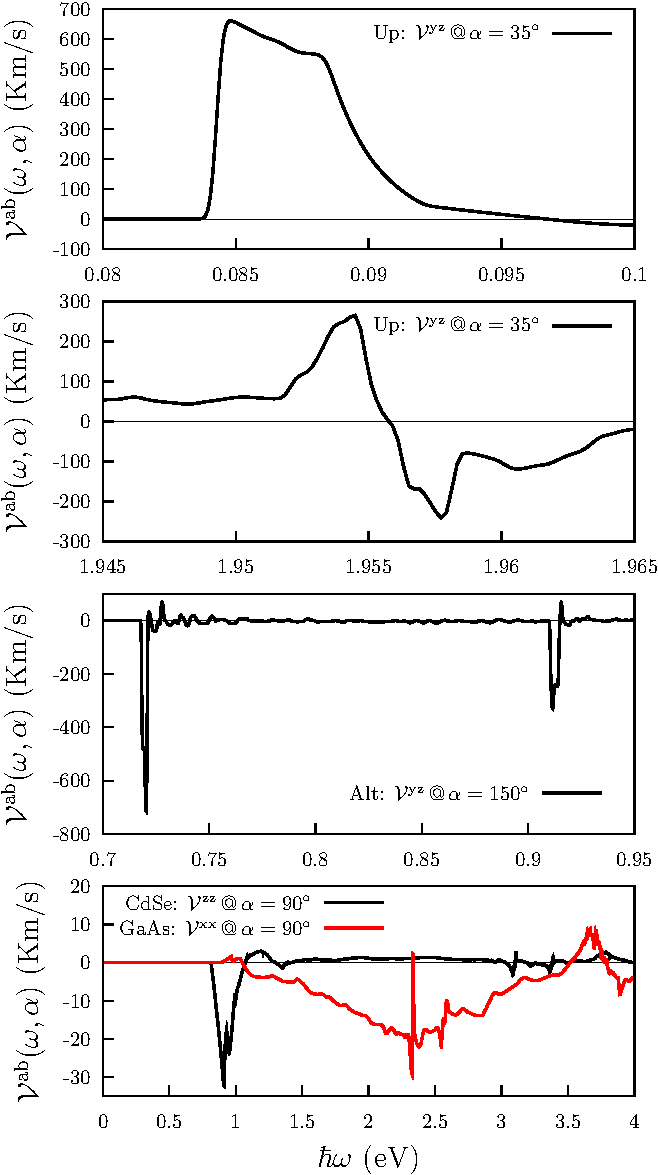
\includegraphics[width=\linewidth]{plots/vab-str-comp}
    
    \caption{Comparison of most intense responses of
    $\mathcal{V}^{\mathrm{ab}}$ for 2D \emph{alt} and \emph{up}, and bulk CdSe
    and GaAs structures and their corresponding polarization angle $\alpha$.}
    \label{fig:vab-str-comp}
\end{figure}

Using the Eq. \eqref{eq:vab-aw}, we calculated the
$\mathcal{V}^{\mathrm{ab}}(\omega,\alpha)$ response for the \emph{up} and
\emph{alt} 2D structures and for the CdSe and GaAs bulk systems; the results
are presented in Fig. \ref{fig:vab-str-comp}. The angle $\alpha$ presented in
the response of each structure is that for which the response is maximized in
each case.
% 
The most intense response corresponds to the \emph{up} structure centered at
0.088\,eV corresponding to the Mid Infrared (MIR) radiation and reaching a spin
velocity of 87.2\,Km/s.
% 
For an energy range from 0.66\,eV to 3.0\,eV, corresponding
to energies of the Near Infrared (NIR) to visible radiation, all
the four structures have contributions of the same order of magnitude.
% 
For this energy range the \emph{up} structure has two peaks centered at
1.94\,eV and 1.97\,eV reaching spin velocities of 22.2\,Km/s and -29.7\,Km/s and the \emph{alt} structure has two peaks centered at 0.72\,eV
and 0.91\,eV reaching spin velocities of -40.2\,Km/s and -32.9\,Km/s,
respectively.
% 
Then, for the bulk structures we have that the CdSe has only one intense
response centered at 0.91\,eV reaching a spin velocity of -26.9\,Km/s, and the
GaAs structure response reaches the maximum for an incoming beam of energy of
2.31\,eV and resulting in a spin velocity of -21.6\,Km/s.
% 
In table \ref{tab:vab-str-comp} we present the comparison of this values for
the 2D and bulk structures; a positive (negative) spin-velocity means that the
velocity moves (anti-)parallel to the electric field.
% 
From the table also we obtain that particularly the 2D \emph{up} structure is
the one with the highest response being between 4 and 5 times more intense than
the corresponding to the bulk structures.


%%%%%%%%%%%%%%%%%%%%%%%%%%%%%%%%%%%%%%%%%%%%%%%%%%%%%%%%%%%%%%%%%%%%%%%%%%%%%%
%%%%%%%%%%%%%%%%%%%%%%%%%%%% Results: Fixing spin %%%%%%%%%%%%%%%%%%%%%%%%%%%%
%%%%%%%%%%%%%%%%%%%%%%%%%%%%%%%%%%%%%%%%%%%%%%%%%%%%%%%%%%%%%%%%%%%%%%%%%%%%%%


\subsection{Fixing spin} % (fold)
\label{sec:res-fixspin}


%%%%%%%%%%%%%%%%%%%%%%%%%%%%%%%%%%%%%%%%%%%%%%%%%%%%%%%%%%%%%%%%%%%%%%%%%%%%%%
%%%%%%%%%%%%%%%%%%%%%%%%%%% Res: fixing spin Up  %%%%%%%%%%%%%%%%%%%%%%%%%%%%%

\begin{figure}[t]
    \centering
    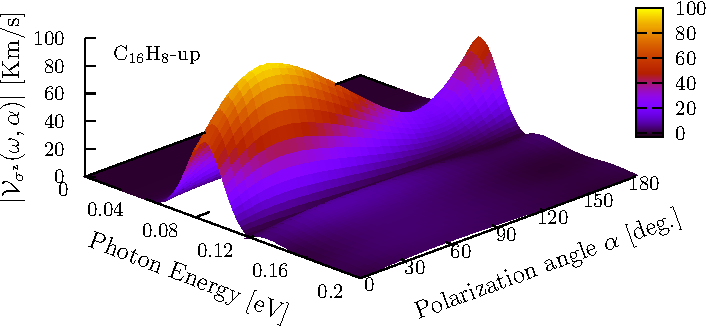
\includegraphics[width=\linewidth]{upplots/up-3d-svaz-1}
    \\
    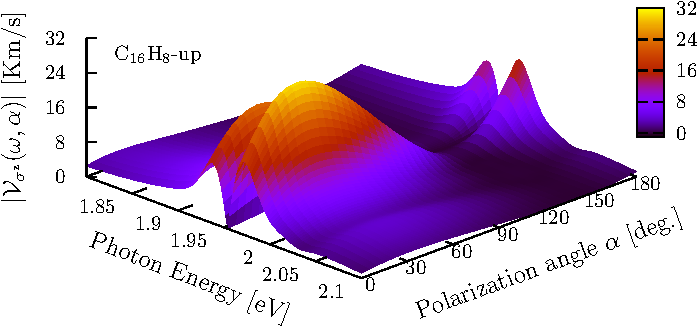
\includegraphics[width=\linewidth]{upplots/up-3d-svaz-2}

    \caption{$|\mathcal{V}_{\sigma^{\mathrm{z}}}(\omega,\alpha)|$ response
    as a function of the photon energy and polarization angle $\alpha$ for the
    \emph{up} structure for two energy ranges. The absolute maxima is located
    for an energy range from 0.08\,eV to 0.10\,eV, in the Far Infrared
    radiation range, and two local maxima from 1.90\,eV to 1.93\,eV and from
    1.96\,eV to 2.0\,eV, in the visible radiation range, all for polarization
    angles between $25^{\circ}$ and $50^{\circ}$.}
    \label{fig:up-3d-vsz}   
\end{figure}

\begin{figure}[t]
    \centering
    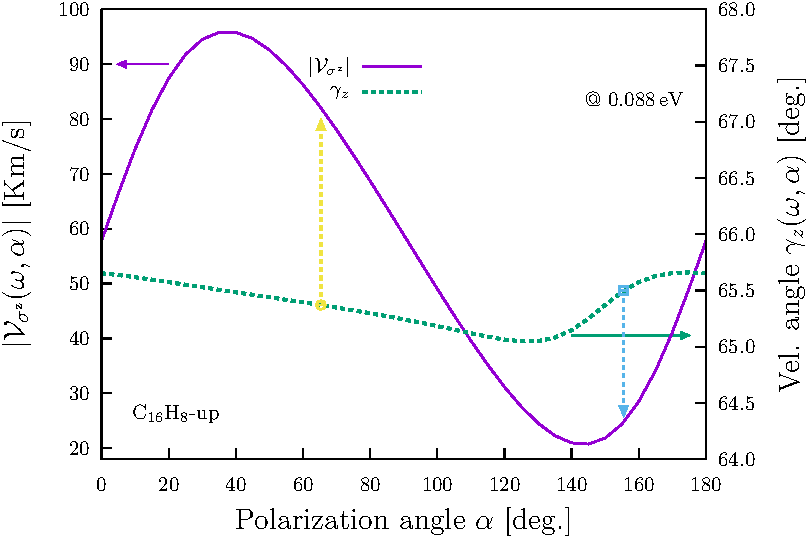
\includegraphics[width=\linewidth]{upplots/up-vaz-rag-1}
    \\
    \vspace{4mm}
    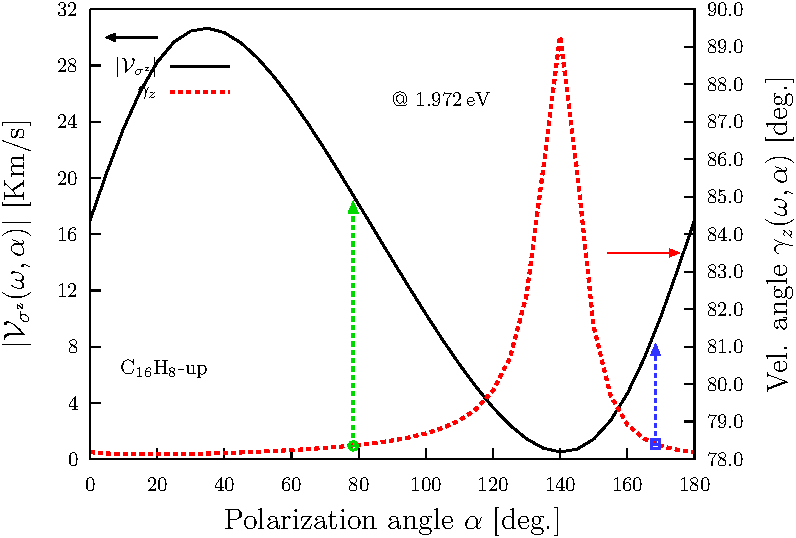
\includegraphics[width=\linewidth]{upplots/up-vaz-rag-2}

    \caption{Most intense response of
    $|\mathcal{V}_{\sigma^{\mathrm{z}}}(\omega,\alpha)|$ (top frames, right
    scale of figs (a) and (b)), the corresponding velocity angle
    $\gamma_{\mathrm{z}}(\omega,\alpha)$ (top frames, right scale), the
    collinear (circled box) and perpendicular (square box) angles, and the two
    components $\mathcal{V}^{\mathrm{xz}}(\omega,\alpha)$ and
    $\mathcal{V}^{\mathrm{yz}}(\omega,\alpha)$ (bottom frames) for the
    \emph{up} structure fixing the energy to 0.088\,eV. }
    \label{fig:up-vaz-rag}
\end{figure}

% %%%%%%%%%%%%%%%%%
% %% 0.0 eV - 0.16 eV  &  1.80 ev - 2.1 ev
% %% Description of UP |V_{s^z}| 3D
% %%%%%%%%%%%%%%%%%

Using Eq. \eqref{eq:vs-mag}, we calculated $|\mathcal{V}_{\sigma^{\mathrm{b}}}
(\omega,\alpha)|$ and made the analysis for the case when the spin is fixed
along $z$ directed perpendicularly to the surface of the \emph{up} and
\emph{alt} structures. Also, using Eq. \eqref{eq:gamma-ang}, we determined the
angle $\gamma_{\mathrm{b}}(\omega,\alpha)$ where the spin-velocity is directed
on the surface of the each structure.
% 

\subsubsection{Up structure}

We present in Fig. \ref{fig:up-3d-vsz} the result of evaluate
$|\mathcal{V}_{\sigma^{\mathrm{z}}} (\omega,\alpha)|$ (Eq. \eqref{eq:vs-mag})
for two energy ranges on the \emph{up} structure.
% 
We obtained that the zone where the maximum response is reached corresponds to
a energy range of the incident beam from 0.084\,eV to 0.093\,eV, in the far
infrared (FIR) and polarization angles $\alpha$ between $30^{\circ}$ and
$45^{\circ}$. Also the two local maxima are held for same beam polarization
angles but for an energy range between 1.90\,eV and 2.05\,eV, in the visible
radiation range.
% %%%%%%%%%%%%%%%%%
% %% 0.0 eV - 0.16 eV
% %% Description of UP |V_{s^z}| & gamma  vs. alpha agle
% %%%%%%%%%%%%%%%%%
In the top panel of Fig. \ref{fig:up-vaz-rag} we present the result of evaluate
Eq. \eqref{eq:vs-mag} (left scale, black solid line) fixing the energy of the
incoming beam to 0.088\,eV for which the response is maximized as shown in the
top panel of Fig. \ref{fig:up-3d-vsz}. The absolute maximum is obtained when
the polarization angle is $\alpha = 40^{\circ}$ resulting in a value of
$|\mathcal{V}_{\sigma^{\mathrm{z}}} (\omega,\alpha)| = 95.8$\,Km/s. This value
comes from the contribution of the components
$\mathcal{V}^{\mathrm{xz}}(\omega,\alpha)=39.8$\,Km/s and
$\mathcal{V}^{\mathrm{yz}}(\omega,\alpha)=87.2$\,Km/s not presented here.
% 
In the same panel we present the corresponding velocity angle
$\gamma_{\mathrm{z}}(\omega,\alpha)$ (right scale, red dashed line), that for
the absolute maximum is $\gamma_{\mathrm{z}}(\omega,\alpha) = 65^{\circ}$. Also
we present two boxes indicating the values for which the angles of the spin
velocity and the polarization angle are parallel (Eq. \ref{eq:gamma-par}, green
circled box), corresponding to $\alpha =
\gamma_{\mathrm{z}\parallel}(\omega,\alpha) = 65.5^{\circ}$; and perpendicular
(Eq. \ref{eq:gamma-perp}, blue squared box), corresponding to $\alpha=155.5^
{\circ}$ and $\gamma_{\mathrm{z}\perp}(\omega,\alpha)=65.5^{\circ}$. The green
and blue dashed arrows are directed from those angles to the respective value
of the response corresponding to
$|\mathcal{V}_{\sigma^{\mathrm{z}}}(\omega,\alpha)| = 82.3$\,Km/s and
$|\mathcal{V}_{\sigma^{\mathrm{z}}}(\omega,\alpha)| = 24.8$\,Km/s.
% 
We also found that the velocity angle is almost constant for all the
polarization angle range having values of $\gamma_{\mathrm{z}}(\omega,\alpha) =
65.5^{\circ}\pm 0.5^{\circ}$.
% 
In the bottom panel of Fig. \ref{fig:up-vaz-rag} we present for the same
structure the result of evaluate Eq. \eqref{eq:vs-mag} fixing now the energy of
the incoming beam to 1.972\,eV for which the response has a local maximum as
shown in the bottom panel of Fig. \ref{fig:up-3d-vsz}. The local maximum is
obtained again when the polarization angle is $\alpha = 40^{\circ}$ resulting
in a value of $|\mathcal{V}_{\sigma^{\mathrm{z}}} (\omega,\alpha)| =
30.3$\,Km/s directed in a velocity angle $\gamma_{\mathrm{z}}(\omega,\alpha) =
78^{\circ}$.
% 
Again, the  green circled box indicates the parallel angles $\alpha =
\gamma_{\mathrm{z}\parallel}(\omega,\alpha) = 78.5^{\circ}$ corresponding to a
spin-velocity $|\mathcal{V}_{\sigma^{\mathrm{z}}}(\omega,\alpha)| =
23.5$\,Km/s indicated with the green arrow
% 
and the blue squared box indicates the perpendicular pair of angles $\alpha =
155.5^ {\circ}$ and $\gamma_{\mathrm{z}\perp}(\omega,\alpha) = 65.5^{\circ}$.
% 
We found again that the velocity angle is almost constant at $78^{\circ}$ and
has variations of $\pm 1^{\circ}$ for polarization angles $0^{\circ} \leq
\alpha \leq 100^{\circ}$.
% 
We also made the analysis for the cases when the spin polarization is directed
along $\mathrm{x}$ and $\mathrm{y}$ but we do not present here the
corresponding plots. For those cases we have that the responses maxima are
obtained for an energy of 0.088\,eV and polarization angle $\alpha=40^{\circ}$
resulting in values of
$|\mathcal{V}_{\sigma^{\mathrm{x}}}(\omega,\alpha)|=37.4$\,Km/s and
$|\mathcal{V}_{\sigma^{\mathrm{y}}}(\omega,\alpha)|=24.8$\,Km/s.

%%%%%%%%%%%%%%%%%%%%%%%%%%%%%%%%%%%%%%%%%%%%%%%%%%%%%%%%%%%%%%%%%%%%%%%%%%%%%%
%%%%%%%%%%%%%%%%%%%%%%%%%%% Res: fixing spin Alt  %%%%%%%%%%%%%%%%%%%%%%%%%%%%

\begin{figure}[tb]
    \centering
    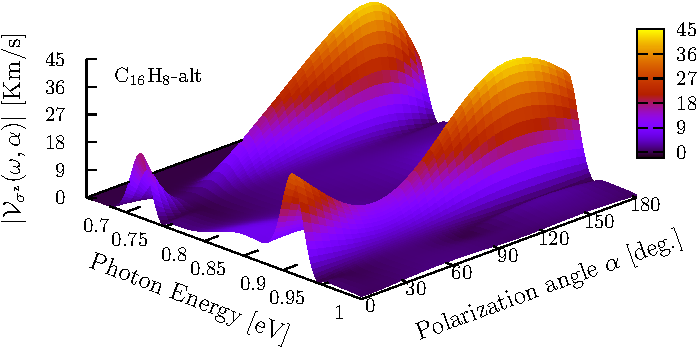
\includegraphics[width=\linewidth]{altplots/alt-3d-svaz}
    \caption{$|\mathcal{V}_{\sigma^{\mathrm{z}}}(\omega,\alpha)|$ response
    as a function of the photon energy and polarization angle $\alpha$  for the
    \emph{alt} structure. The local and the absolute maxima are located in the
    energy ranges from 0.67\,eV to 0.73\,eV and from 0.90\,eV to 0.93\,eV,
    respectively, and both in the Near Infrared and for polarization angles
    between $120^{\circ}$ and $150^{\circ}$.}
    \label{fig:alt-3d-vsb}
\end{figure}

\begin{figure}[t]
    \centering
    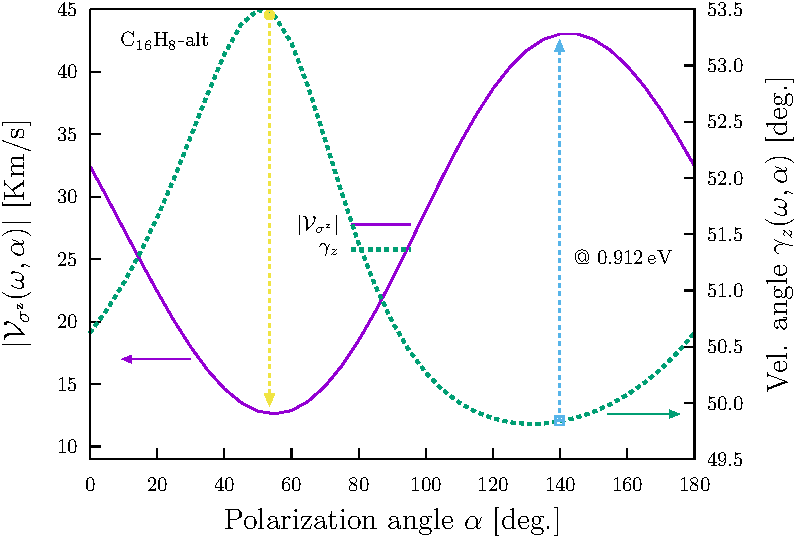
\includegraphics[width=\linewidth]{altplots/alt-vaz-rag}
    \caption{Most intense response of
    $|\mathcal{V}_{\sigma^{\mathrm{z}}}(\omega,\alpha)|$ (top frame, left
    scale) the corresponding velocity angle $\gamma_{\mathrm{z}}(\omega)$ (top
    frame, right scale), the collinear (circled box) and perpendicular (square
    box) angles, and the two components $\mathcal{V}^{\mathrm{xz}}(\omega)$ and
    $\mathcal{V}^{\mathrm{yz}}(\omega)$ (bottom frame) for the \emph{alt}
    structure fixing the energy to 0.912\,eV.}
    \label{fig:alt-vaz-rag}
\end{figure}

% %%%%%%%%%%%%%%%%%
% %% 0.0 eV - 0.16 eV  &  1.80 ev - 2.1 ev
% %% Description of ALT |V_{s^z}| 3D
% %%%%%%%%%%%%%%%%%

\subsubsection{Alt structure}

We present in Fig. \ref{fig:alt-3d-vsb} the result of evaluate
$|\mathcal{V}_{\sigma^{\mathrm{z}}} (\omega,\alpha)|$ (Eq. \eqref{eq:vs-mag})
on the \emph{alt} structure.
% 
We obtained that the zone where the maximum response is reached corresponds to
energies from 0.90\,eV to 0.93\,eV and a local maximum is obtained
for energies between 0.67\,eV and 0.75\,eV both located in the FIR radiation
range and for polarization angles between $120^{\circ}$ and $150^{\circ}$.
% %%%%%%%%%%%%%%%%%
% %% 0.0 eV - 0.16 eV
% %% Description of ALT |V_{s^z}| & gamma  vs. alpha agle
% %%%%%%%%%%%%%%%%%
In the top panel of Fig. \ref{fig:up-vaz-rag} we present the result of evaluate
Eq. \eqref{eq:vs-mag} (left scale, black solid line) fixing the energy to
0.912\,eV for which the response is maximized as shown in the
top panel of Fig. \ref{fig:up-3d-vsz}. The absolute maximum is obtained when
the polarization angle is $\alpha = 40^{\circ}$ resulting in a value of
$|\mathcal{V}_{\sigma^{\mathrm{z}}} (\omega,\alpha)| = 43.0$\,Km/s.
% 
In the same panel we present the velocity angle
$\gamma_{\mathrm{z}}(\omega,\alpha)$ (right scale, red dashed line), that for
the absolute maximum is $\gamma_{\mathrm{z}}(\omega,\alpha) = 145^{\circ}$.
% 
As explained for the previous case, the green circled box indicates the
parallel pair of angles $\alpha = \gamma_{\mathrm{z}\parallel}(\omega,\alpha) =
53.5^{\circ}$ with a corresponding value
$|\mathcal{V}_{\sigma^{\mathrm{z}}}(\omega,\alpha)| = 12.7$\,Km/s indicated
with the green arrow, and the blue square box indicates the perpendicular pair
of angles, $\alpha=140^{\circ}$ and
$\gamma_{\mathrm{z}\perp}(\omega,\alpha)=50^{\circ}$, with a value of
$|\mathcal{V}_{\sigma^{\mathrm{z}}} (\omega,\alpha)|=43.0$\,Km/s indicated with
the blue arrow.
% 
We also have that the velocity angle is centered at $51.5^{\circ}$ having
variations of $\pm 2^{\circ}$ for the polarization angle range $0^{\circ} \leq
\alpha \leq 180^{\circ}$.
% 
Again, for the cases in which the spin polarization is parallel to the surface
of the \emph{alt} structure was calculated but the plots are not presented
here. The absolute maxima for the cases when the spin polarization are directed
in the $x$ and $y$ direction are obtained for an energy of 0.912\,eV and
polarization angle $\alpha=145^{\circ}$ resulting in values of
$|\mathcal{V}_{\sigma^{\mathrm{x}}}(\omega,\alpha)| = 27.1$\,Km/s and
$|\mathcal{V}_{\sigma^{\mathrm{y}}}(\omega,\alpha)| = 33.2$\,Km/s.


%%%%%%%%%%%%%%%%%%%%%%%%%%%%%%%%%%%%%%%%%%%%%%%%%%%%%%%%%%%%%%%%%%%%%%%%%%%%%%
%%%%%%%%%%%%%%%%%%%%%%%%%% Results: Fixing velocity %%%%%%%%%%%%%%%%%%%%%%%%%%
%%%%%%%%%%%%%%%%%%%%%%%%%%%%%%%%%%%%%%%%%%%%%%%%%%%%%%%%%%%%%%%%%%%%%%%%%%%%%%


\subsection{Fixing velocity} % (fold)
\label{sec:res-fixvel}


%%%%%%%%%%%%%%%%%%%%%%%%%%%%%%%%%%%%%%%%%%%%%%%%%%%%%%%%%%%%%%%%%%%%%%%%%%%%%%
%%%%%%%%%%%%%%%%%%%%%%%%%%% Res: fixin vel Up  %%%%%%%%%%%%%%%%%%%%%%%%%%%%%%%

Now, using the Eq. \eqref{eq:vv-mag}, we calculated the
$|\mathcal{V}^{\mathrm{a}} (\omega,\alpha)|$ for the case when the velocity is
fixed in the $x$ and $y$ direction on the surface of the \emph{up} and
\emph{alt} structures. Also, using the Eqns. \eqref{eq:polar-ang} and 
\eqref{eq:azimuthal-ang}, we determined the polar $\theta_{\mathrm{a}}
(\omega,\alpha)$ and azimuthal $\varphi_{\mathrm{a}} (\omega,\alpha)$ angles
corresponding to the direction of the spin.

\subsubsection{Up structure}

\begin{figure}[t]
    \centering
    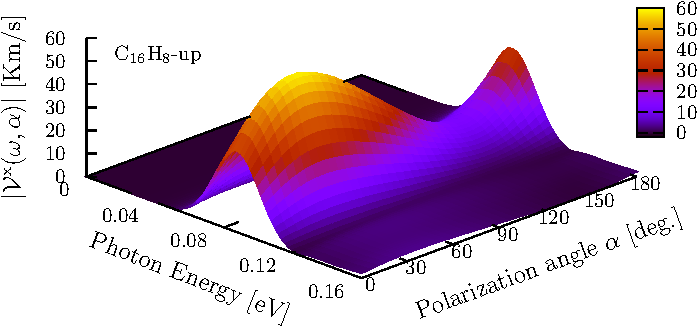
\includegraphics[width=\linewidth]{upplots/up-3d-vxb-1}
    \\
    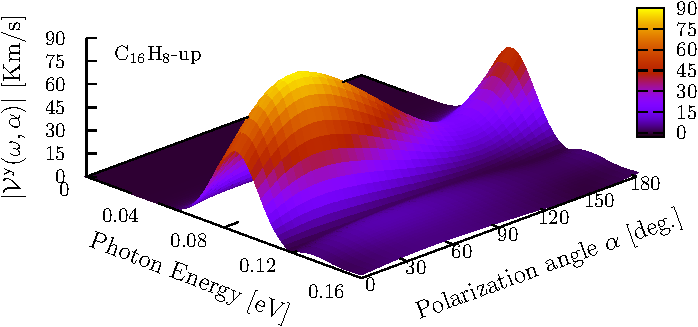
\includegraphics[width=\linewidth]{upplots/up-3d-vyb-1}
    
    \caption{ $|\mathcal{V}^{\mathrm{x}}(\omega,\alpha)|$ and
    $|\mathcal{V}^{\mathrm{y}}(\omega,\alpha)|$responses as a function of the
    photon energy and polarization angle $\alpha$ for the \emph{up} structure.
    The absolute maxima of both are localized in the energy range from 0.08\,eV
    to 0.10\,eV, in the Far  Infrared, and for polarization angles from
    $25^{\circ}$ to $50^{\circ}$.}
    \label{fig:up-3d-vva-1}
\end{figure}
\begin{figure}[t]
    \centering
    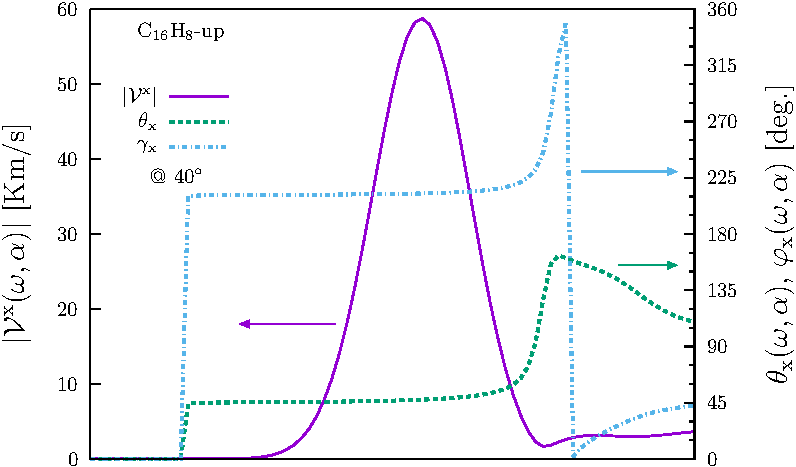
\includegraphics[width=\linewidth]{upplots/up-vxb-rtp-m1}
    \\ \vspace{4mm}
    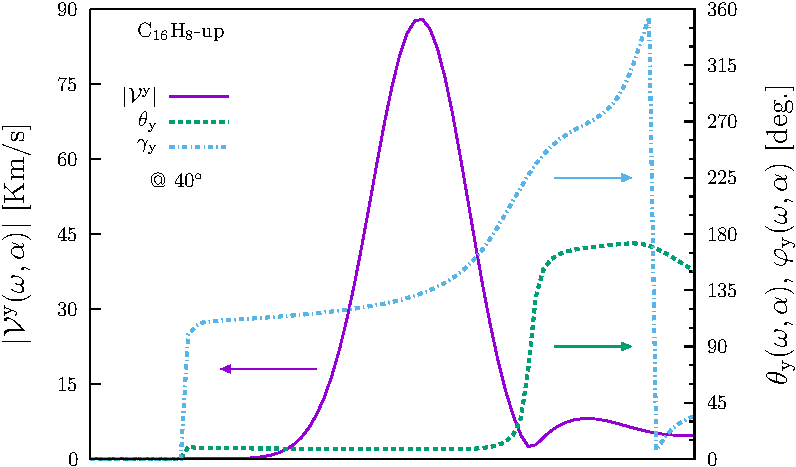
\includegraphics[width=\linewidth]{upplots/up-vyb-rtp-m1}
    
    \caption{Most intense response of
    $|\mathcal{V}^{\mathrm{x}}(\omega,\alpha)|$ and
    $|\mathcal{V}^{\mathrm{y}}(\omega,\alpha)|$ (top frames left scale of Figs.
    (a) and (b)), the corresponding polar $\varphi$ and azimuthal $\theta$
    angles (top frames right scale), and the corresponding three components
    (bottom frames) for the \emph{up} structure fixing the polarization angle
    to $\alpha=40^{\circ}$ to maximize the response.}
    \label{fig:up-vab-comp-rtp-1}
\end{figure}
% %%%%%%%%%%%%%%%%%
% %% 0.0 eV - 0.16 eV
% %% Description of UP |V^{a}| 3D
% %%%%%%%%%%%%%%%%%
In top and bottom panels of Fig. \ref{fig:up-3d-vva-1} we present the
result of evaluate Eq. \eqref{eq:vv-mag} for the
\emph{up} structure fixing the velocity in the $x$ and $y$ direction.
%
From this figure we can see that the two absolute maxima are obtained for
energies between 0.084\,eV and 0.093\,eV, in the FIR, and polarization angles
between $30^ {\circ}$ and $45^{\circ}$.
% 
In the top and bottom panels of Fig. \ref{fig:up-vab-comp-rtp-1} we present $|
\mathcal{V}^{\mathrm{x}} (\omega,\alpha)|$ and $|\mathcal{V}^{\mathrm{y}}
(\omega,\alpha)|$ (left scale, black solid line) fixing the polarization angle
to $\alpha=40^{\circ}$ for which the responses have absolute maxima of
58.7\,Km/s and 87.9\,Km/s, respectively, for an energy of 0.088\,eV.
% 
In same panels we present the corresponding polar (right scale, red dashed
line) and azimuthal (right scale, blue dashed line) spin polarization angles
that have values of $\theta_{\mathrm{x}}(\omega,\alpha) = 47^{\circ}$,
$\varphi_{\mathrm{x}}(\omega,\alpha) = 212^{\circ}$, $\theta_{\mathrm{y}}
(\omega,\alpha) = 8^{\circ}$ and $\varphi_{\mathrm{y}} (\omega,\alpha) =
133^{\circ}$. In this way, the spin is directed upward the third Cartesian
quadrant of the $xy$ plane when it moves along $x$, and is directed almost
perpendicularly over the $xy$ plane when it moves along $y$.
% 
Also from this figure we have that when the spin moves along $x$ the angles are
almost constant for the peak of the response having variations of $\pm
2^{\circ}$ but when the spin moves along $y$ the azimuthal angle changes from
$99^{\circ}$ to $176^{\circ}$

\begin{figure}[t]
    \centering
    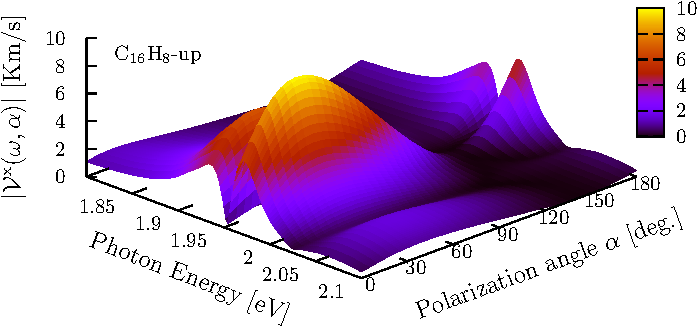
\includegraphics[width=\linewidth]{upplots/up-3d-vxb-2}
    \\
    
\includegraphics[width=\linewidth]{upplots/up-3d-vyb-2}
    
    \caption{$|\mathcal{V}^{\mathrm{x}}(\omega,\alpha)|$ (top panel) and
    $|\mathcal{V}^{\mathrm{y}}(\omega,\alpha)|$ (bottom panel)  as a function
    of the photon energy and polarization angle $\alpha$ for the \emph{up}
    structure. Two local maxima of both responses are localized in the energy
    range from 1.90\,eV to 1.93\,eV and from 1.96\,eV to 2.0\,eV, in the
    visible radiation range, and for polarization angles between $25^{\circ}$
    and $50^{\circ}$.}
    \label{fig:up-3d-vva-2}
\end{figure}
\begin{figure}[t]
    \centering
    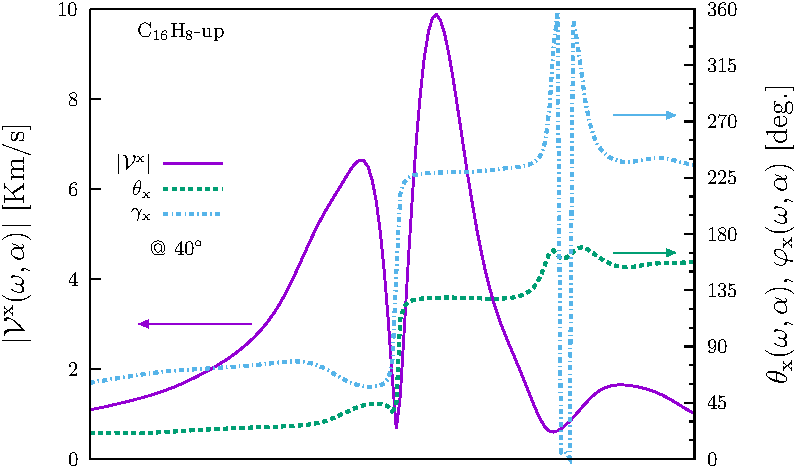
\includegraphics[width=\linewidth]{upplots/up-vxb-rtp-m2}
    \\ \vspace{4mm}
    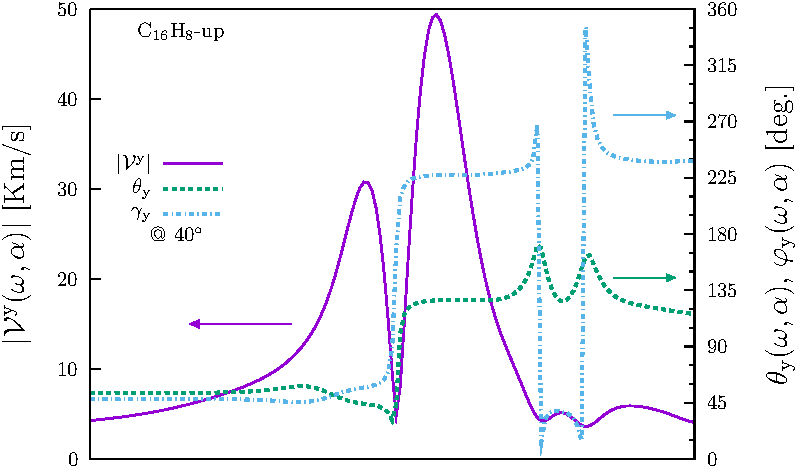
\includegraphics[width=\linewidth]{upplots/up-vyb-rtp-m2}
    
    \caption{Intense response of
    $|\mathcal{V}^{\mathrm{x}}(\omega,\alpha)|$ and
    $|\mathcal{V}^{\mathrm{y}}(\omega,\alpha)|$ (top frames left scale of Figs.
    (a) and (b)), the corresponding polar $\varphi$ and azimuthal $\theta$
    angles (top frames right scale), and the corresponding three components
    (bottom frames) for the \emph{up} structure fixing the polarization angle
    to $\alpha=40^{\circ}$ to maximize the response.}

    \label{fig:up-vab-comp-rtp-2}
\end{figure}
% %%%%%%%%%%%%%%%%%
% %% 1.80 eV - 2.10 eV
% %% Description of UP |V^{a}| 3D
% %%%%%%%%%%%%%%%%%

In top and bottom panels of Fig. \ref{fig:up-3d-vva-2} we present the
result of evaluate Eq. \eqref{eq:vv-mag} for the same structure fixing the
velocity in the $x$ and $y$ direction for other range of energies that present
a intense response.
% 
From this figure we can see that the two local maxima are obtained for energies
between 1.80\,eV and 2.10\,eV, in the range of visible radiation, and
polarization angles between $30^ {\circ}$ and $45^{\circ}$.
% 
From the top and bottom panels of Fig. \ref{fig:up-vab-comp-rtp-2} we have that
$|\mathcal{V}^{\mathrm{x}} (\omega,\alpha)| =  9.8$\,Km/s and
$|\mathcal{V}^{\mathrm{y}} (\omega,\alpha)| = 49.3$\,Km/s fixing the
polarization angle to $\alpha=40^{\circ}$ and the beam energy to 1.932\,eV.
% 
In same panels we present the corresponding polar and azimuthal spin
polarization angles that have values of $\theta_{\mathrm{x}}(\omega,\alpha) =
129^{\circ}$, $\varphi_{\mathrm{x}}(\omega,\alpha) = 229^{\circ}$,
$\theta_{\mathrm{y}} (\omega,\alpha) = 127^{\circ}$ and $\varphi_{\mathrm{y}}
(\omega,\alpha) = 227^{\circ}$ being constant all of them in the peak of the
local maxima. Then, the spin is directed downward the third Cartesian quadrant
of the $xy$ plane when it moves along $x$ and $y$ directions.

%%%%%%%%%%%%%%%%%%%%%%%%%%%%%%%%%%%%%%%%%%%%%%%%%%%%%%%%%%%%%%%%%%%%%%%%%%%%%%
%%%%%%%%%%%%%%%%%%%%%%%%%%% Res: fixin vel Alt  %%%%%%%%%%%%%%%%%%%%%%%%%%%%%%%

\subsubsection{Alt structure}

\begin{figure}[tb]
    \centering
    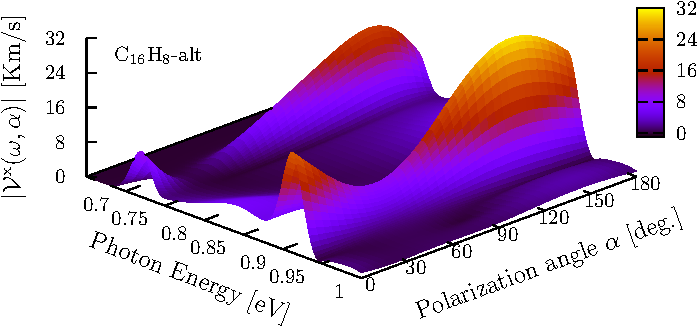
\includegraphics[width=\linewidth]{altplots/alt-3d-vxb}
    \\
    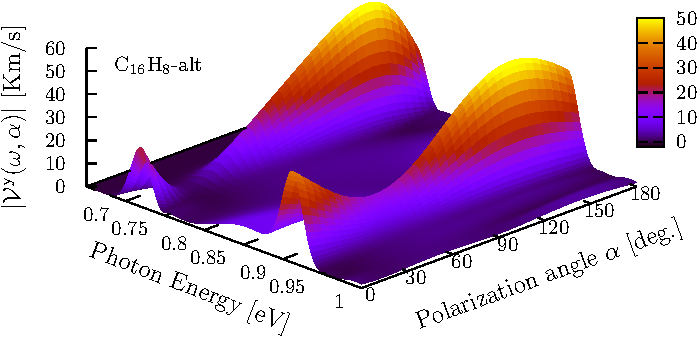
\includegraphics[width=\linewidth]{altplots/alt-3d-vyb}
    
    \caption{$|\mathcal{V}^{\mathrm{x}}(\omega,\alpha)|$ (top panel) and
    $|\mathcal{V}^{\mathrm{y}}(\omega,\alpha)|$ (bottom panel)  as a function
    of the photon energy and polarization angle $\alpha$ for the \emph{alt}
    structure. The local and the absolute maxima are located in the energy
    ranges from 0.67\,eV to 0.73\,eV and from 0.90\,eV to 0.93\,eV,
    respectively, and both in the Near Infrared and for polarization angles
    between $120^{\circ}$ and $150^{\circ}$.}
    \label{fig:alt-3d-vva}
\end{figure}

\begin{figure}[tb]
    \centering
    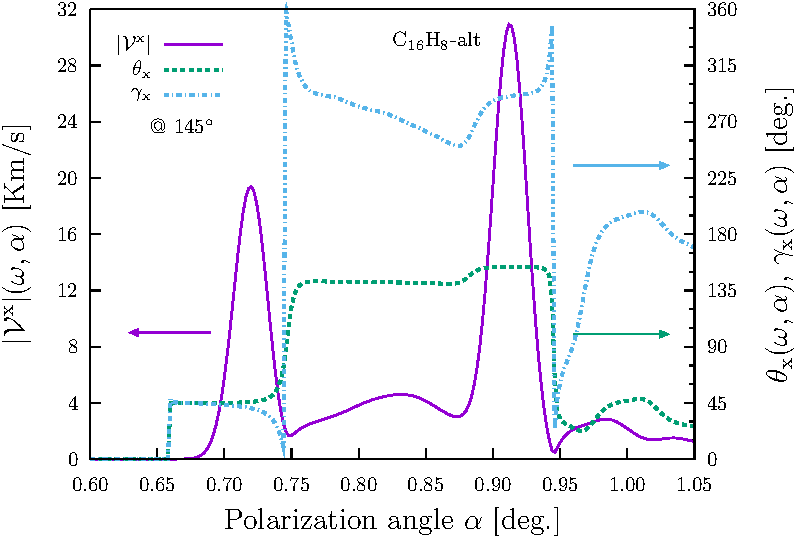
\includegraphics[width=\linewidth]{altplots/alt-vxb-rtp-m}
    \\ \vspace{4mm}
    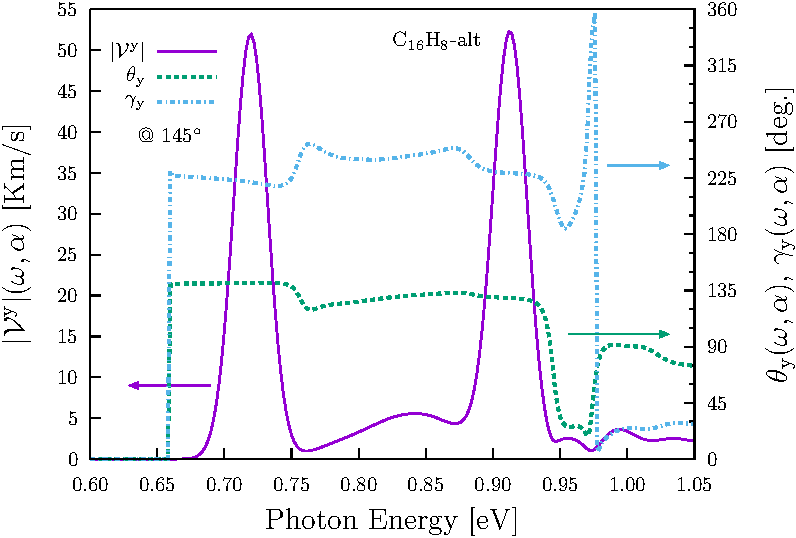
\includegraphics[width=\linewidth]{altplots/alt-vyb-rtp-m}

    \caption{Most intense response of
    $|\mathcal{V}^{\mathrm{x}}(\omega,\alpha)|$ and
    $|\mathcal{V}^{\mathrm{y}}(\omega,\alpha)|$ (top frames left scale of Figs.
    (a) and (b)), the corresponding polar $\varphi$ and azimuthal $\theta$
    angles (top frames right scale), and the corresponding three components
    (bottom frames) for the \emph{alt} structure fixing the polarization angle
    to $\alpha=145^{\circ}$ to maximize the response.}
    \label{fig:alt-vab-comp-rtp}
\end{figure}

% %%%%%%%%%%%%%%%%%
% %% Description of ALT |V^{a}| 3D
% %%%%%%%%%%%%%%%%%

In top and bottom panels of Fig. \ref{fig:alt-3d-vva} we present the
result of evaluate Eq. \eqref{eq:vv-mag} for the
\emph{up} structure fixing the velocity in the $x$ and $y$ direction.
% 
From this figure we have that the relative maxima for the spin velocity along
$x$ and $y$ are obtained for energies between 0.70\,eV to 0.75\,eV and the
absolute maxima are obtained for energies between 0.90\,eV and 0.93\,eV, all
cases in the NIR radiation, and polarization angles between 120$^{\circ}$ and
150$^{\circ}$.
% 
From the top and bottom panels of Fig. \ref{fig:alt-vab-comp-rtp} we have that
that the local maxima are $|\mathcal{V}^{\mathrm{x}} (\omega,\alpha)| =
19.4$\,Km/s and $|\mathcal{V}^{\mathrm{y}} (\omega,\alpha)| = 51.9$\,Km/s
fixing the energy to 0.720\,eV and the absolute maxima are
$|\mathcal{V}^{\mathrm{x}} (\omega,\alpha)| = 30.9$\,Km/s and
$|\mathcal{V}^{\mathrm{y}} (\omega,\alpha)| = 52.2$\,Km/s fixing the energy to
0.912\,eV all for a polarization angle $\alpha=145^{\circ}$.
% 
The corresponding polar and azimuthal angles for the local maxima are
$\theta_{\mathrm{x}} (\omega,\alpha) = 46^{\circ}$, $\varphi_{\mathrm{x}}
(\omega,\alpha) = 41^{\circ}$, $\theta_{\mathrm{y}} (\omega,\alpha) =
141^{\circ}$ and $\varphi_{\mathrm{y}} (\omega,\alpha) = 222^{\circ}$ being the
spin directed over the first Cartesian quadrant of the $xy$ plane when the spin
velocity is directed along $x$ and directed downward the third Cartesian
quadrant when the spin velocity is directed along $y$. Finally, the angles for
the absolute maxima are $\theta_{\mathrm{x}}(\omega,\alpha) = 154^{\circ}$,
$\varphi_{\mathrm{x}} (\omega,\alpha) = 290^{\circ}$, $\theta_{\mathrm{y}}
(\omega,\alpha) = 129^{\circ}$ and $\varphi_{\mathrm{y}} (\omega,\alpha) =
229^{\circ}$ being the spin polarization directed downward the fourth Cartesian
quadrant when the spin velocity is directed along $x$ and downward the third
Cartesian quadrant when the spin velocity is directed along $y$.

%%%%%%%%%%%%%%%%%%%%%%%%%%%%%%%%%%%%%%%%%%%%%%%%%%%%%%%%%%%%%%%%%%%%%%%%%%%%%%
%%%%%%%%%%%%%%%%%%%%%%%%%% Res: Layer-by-layer  %%%%%%%%%%%%%%%%%%%%%%%%%%%%%%
%%%%%%%%%%%%%%%%%%%%%%%%%%%%%%%%%%%%%%%%%%%%%%%%%%%%%%%%%%%%%%%%%%%%%%%%%%%%%%

\subsection{Layer-by-layer analysis} % (fold)
\label{sec:res-layer_by_layer_analysis}


As mentioned before in in the beginning of this section the \emph{up} and
\emph{alt} structures presented here was divided into layers to analyze the
layer-by-layer contribution for $|\mathcal{V}_{\sigma^{\mathrm{b}}}
(\omega,\alpha)|$ and $|\mathcal{V}^{\mathrm{a}} (\omega,\alpha)|$. 
% 
In Tables \ref{tab:up-unitcell} and \ref{tab:alt-unitcell} we present the layer
division needed to calculate the layer-by-layer contribution for the
$|\mathcal{V}_{\sigma^{\mathrm{b}}}(\omega,\alpha)|$ and
$|\mathcal{V}^{\mathrm{a}}(\omega,\alpha)|$ presented in Eqns.
\eqref{eq:vs-layer} and \eqref{eq:vv-layer}. The \emph{up} structure was
divided in two layers, the first comprised of the top hydrogen atoms denoted by
the number 1 in Table \ref{tab:up-unitcell} and in the Fig. \ref{fig:up-struc}
and the second comprised of carbon atoms and denoted by the number 2. The
\emph{alt} structure was divided in six layers denoted with numbers from 1 to 6
in Table \ref{tab:alt-unitcell} and in Fig. \ref{fig:alt-struc}. The first and
sixth layers correspond to hydrogen atoms in the top and bottom positions and
from the second to the fifth correspond to carbon atoms placed in different
positions.
% 
Here we present the decomposition only for $|\mathcal{V}_{\sigma^{\mathrm{z}}}
(\omega,\alpha)|$ and for the corresponding components of the \emph{up}
structure in Figs.
% 
\ref{fig:up-vsz-lay-1} and \ref{fig:up-vsz-lay-2} and for the \emph{alt}    
structure in Fig. \ref{fig:alt-vsz-lay}. 
% 
% The $|\mathcal{V}_{\sigma^{\mathrm{z}}}(\omega,\alpha)|$ response presented
% in those figures is the same than the presented in top frames of Figs.
% \ref{fig:up-vaz-rag} and \ref{fig:alt-vaz-rag} but now compared with the
% layered responses.
% 
\begin{figure}[t]
    \centering
    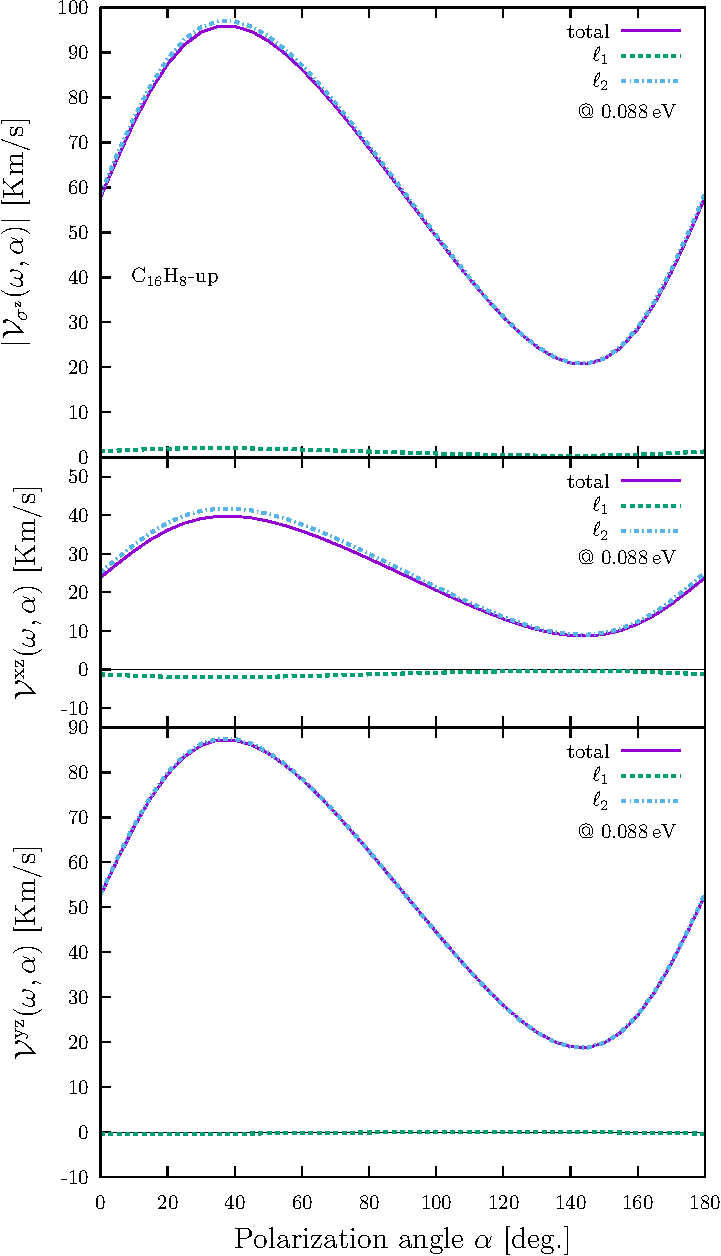
\includegraphics[width=\linewidth]{upplots/up-svaz-lay-1}
    
    \caption{Layer-by-layer contribution of the
    $|\mathcal{V}_{\sigma^{\mathrm{z}}}(\omega,\alpha)|$ response (top frame)
    for the \emph{up} structure as a function of the polarization angle
    $\alpha$ for the energy fixed to 0.088\,eV for which the absolute maximum
    is obtained.
    % 
    The corresponding layered contributions for the
    $\mathcal{V}^{\mathrm{xz}}(\omega,\alpha)$ and
    $\mathcal{V}^{\mathrm{zy}}(\omega,\alpha)$ components are presented in the
    central and bottom frames.}
    \label{fig:up-vsz-lay-1}
\end{figure}

\begin{figure}[t]
    \centering
    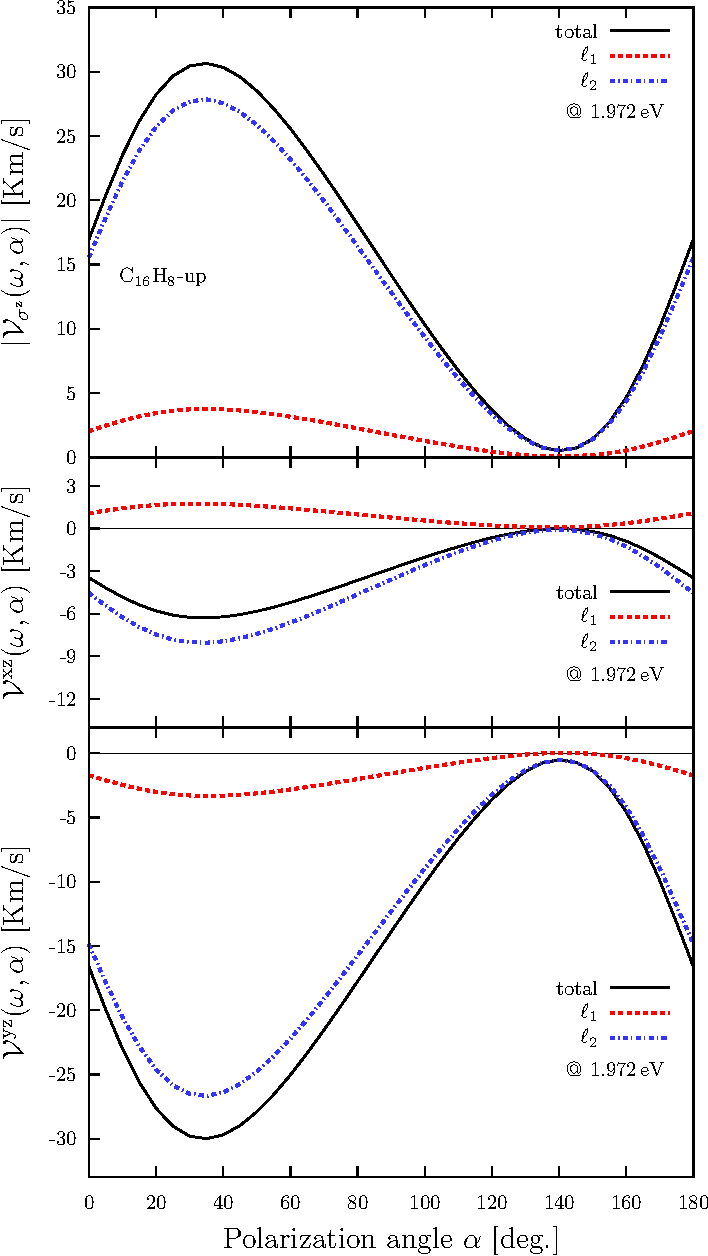
\includegraphics[width=\linewidth]{upplots/up-svaz-lay-2}
    
    \caption{Layer-by-layer contribution of the
    $|\mathcal{V}_{\sigma^{\mathrm{z}}}(\omega,\alpha)|$ response (top frame)
    for the \emph{up} structure as a function of the polarization angle
    $\alpha$ for the energy fixed to 1.972\,eV for which a local maximum is
    obtained.
    % 
    The corresponding layered contributions for the
    $\mathcal{V}^{\mathrm{xz}}(\omega,\alpha)$ and
    $\mathcal{V}^{\mathrm{zy}}(\omega,\alpha)$ components are presented in the
    central and bottom frames.}
    \label{fig:up-vsz-lay-2}
\end{figure}

\begin{figure}[t]
    \centering
    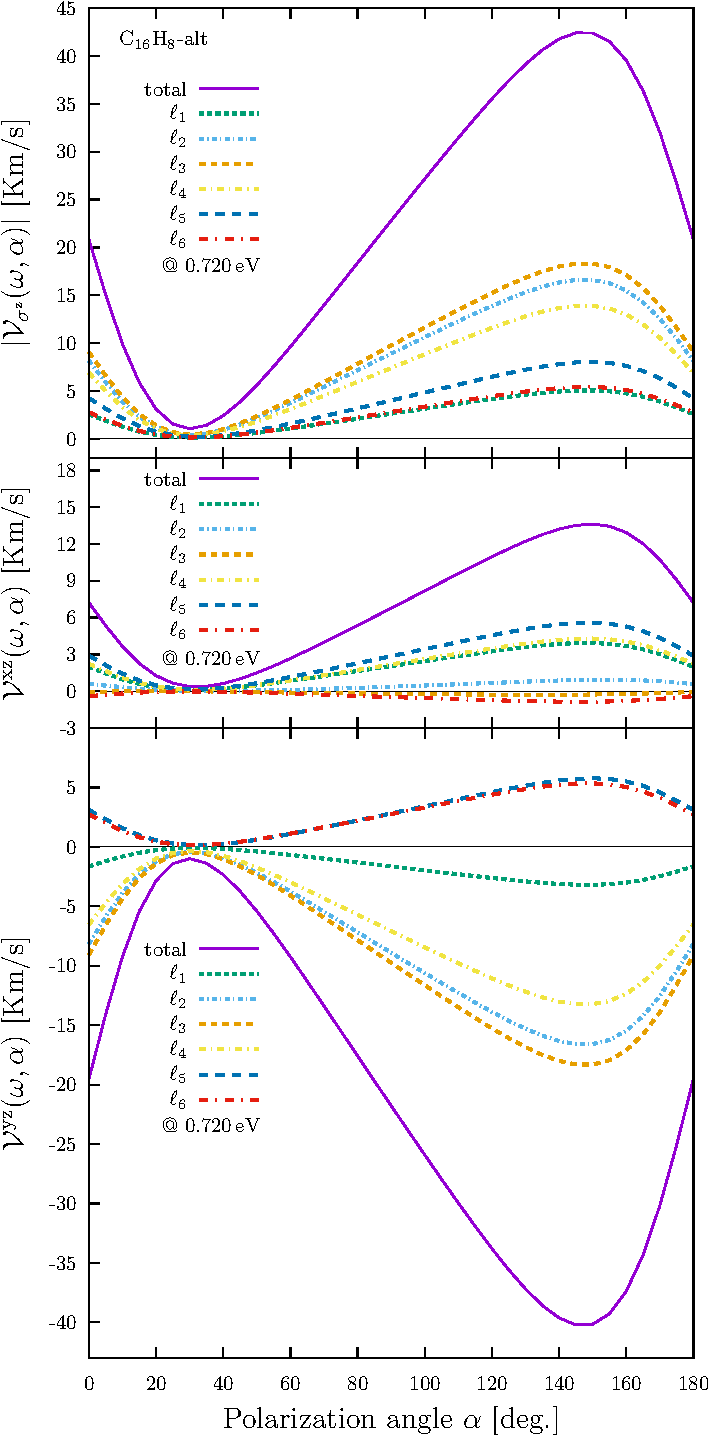
\includegraphics[width=\linewidth]{altplots/alt-svaz-lay-1}
    
\caption{Layer-by-layer contribution of the
    $|\mathcal{V}_{\sigma^{\mathrm{z}}}(\omega,\alpha)|$ response (top frame)
    for the \emph{alt} structure as a function of the polarization angle
    $\alpha$ for the energy fixed to 0.720\,eV.
    % 
    The corresponding layered contributions for the
    $\mathcal{V}^{\mathrm{xz}}(\omega,\alpha)$ and
    $\mathcal{V}^{\mathrm{zy}}(\omega,\alpha)$ components are presented in the
    central and bottom frames.}
    \label{fig:alt-vsz-lay}
\end{figure}
% 

% %%%%%%%%%%%%%%%%
% %% Description of Up layer |V_{s^z}|
% %%%%%%%%%%%%%%%%
From the central and bottom frames of Fig. \ref{fig:up-vsz-lay-1} we have that
when the energy is fixed to 0.088\,eV almost all the response of the
$\mathcal{V}^{\mathrm{xz}}(\omega,\alpha)$ component comes from the second
layer comprised by carbon atoms having a minimal reduction produced by the
hydrogen layer.
% 
Also, the $\mathcal{V}^{\mathrm{yz}}(\omega,\alpha)$ response, presented in
bottom frame of same figure, is produced only by the carbon layer. This result
in a total response $|\mathcal{V}_{\sigma^{\mathrm{z}}}(\omega,\alpha)| =
95.8$\,Km/s coming from the carbon layer and being minimally reduced by the
hydrogen layer as shown in the top frame of this figure for a fixed
polarization angle $\alpha = 40^{\circ}$.
% 
Now, for the same structure but now fixing the energy to 1.972\,eV we have from
the central frame of Fig. \ref{fig:up-vsz-lay-2} that the the carbon layer
produces the response of the $\mathcal{V}^{\mathrm{zx}}(\omega,\alpha)$
component being decreased by the hydrogen layer. Opposite to that, in the
bottom frame of same figure we obtained that the response of the carbon and
hydrogen layer are not inverse and then contributing both to the total response
of $\mathcal{V}^{\mathrm{yz}}(\omega,\alpha)$. Then, in the top frame of this
figure we have that the major contribution to the
$|\mathcal{V}_{\sigma^{\mathrm{z}}}(\omega,\alpha)|$ response comes from the
carbon layer with but being in this case reinforced by the contribution of the
hydrogen layer and resulting in a value of 30.3\,Km/s.
% %%%%%%%%%%%%%%%%
% %% Description of ALT layer |V^{yz}|
% %%%%%%%%%%%%%%%%
Finally, for the \emph{alt} structure we have that, for the response $|
\mathcal{V}_{\sigma^{\mathrm{z}}} (\omega,\alpha)|$ when the energy is fixed to
0.720\,eV the six layers contribute with similar magnitudes. 
% 
We found that for the $\mathcal{V}^{\mathrm{xz}} (\omega,\alpha)$ and
$\mathcal{V}^{\mathrm{yz}} (\omega,\alpha)$ components the top hydrogen layer
response, denoted by $\ell_{1}$, cancels partially the the bottom hydrogen
layer response, denoted by $\ell_{6}$;
% 
a similar behavior occurs in the component $\mathcal{V}^{\mathrm{xz}}
(\omega,\alpha)$ for the third and fourth carbon layers and in the component
$\mathcal{V}^{\mathrm{yz}} (\omega,\alpha)$ for the second and fifth carbon
layers.
% 
This result in a total response $\mathcal{V}^{\mathrm{xz}}(\omega,\alpha) =
42.4$\,Km/s for a fixed polarization angle $\alpha = 145^{\circ}$.
% 
Then, for this analysis we found that the $|\mathcal{V}_{\sigma^{\mathrm{z}}} 
(\omega,\alpha)|$ and in general, $\mu^{\mathrm{abcd}} (\omega)$ responses are
very susceptible to the symmetry of the system. The \emph{up} structure is 
\emph{more} non-centrosymmetric than the \emph{alt} structure and then the
response is quite larger.


%%%%%%%%%%%%%%%%%%%%%%%%%%%%%%%%%%%%%%%%%%%%%%%%%%%%%%%%%%%%%%%%%%%%%%%%%%%%%%
%%%%%%%%%%%%%%%%%%%%%%%%%%%%%%%%%%%%%%%%%%%%%%%%%%%%%%%%%%%%%%%%%%%%%%%%%%%%%%
%%%%%%%%%%%%%%%%%%%%%%%%%%                          %%%%%%%%%%%%%%%%%%%%%%%%%%
%%%%%%%%%%%%%%%%%%%%%%%%%%   C O N C L U S I O N S  %%%%%%%%%%%%%%%%%%%%%%%%%%
%%%%%%%%%%%%%%%%%%%%%%%%%%                          %%%%%%%%%%%%%%%%%%%%%%%%%%
%%%%%%%%%%%%%%%%%%%%%%%%%%%%%%%%%%%%%%%%%%%%%%%%%%%%%%%%%%%%%%%%%%%%%%%%%%%%%%
%%%%%%%%%%%%%%%%%%%%%%%%%%%%%%%%%%%%%%%%%%%%%%%%%%%%%%%%%%%%%%%%%%%%%%%%%%%%%%


%%%%%%%%%%%%%%%%%%%%%%%%%%%%%%%%%%%%%%%%%%%%%%%%%%%%%%%%%%%%%%%%%%%%%%%%%%%%%%
%%%%%%%%%%%%%%%%%%%%%%%%%%%%%%%%%%%%%%%%%%%%%%%%%%%%%%%%%%%%%%%%%%%%%%%%%%%%%%

\section{Conclusions} % (fold)
\label{sec:conclusions}

We have performed an \emph{ab initio} calculation for the SVI by one-photon
absorption of linearly polarized light in the \emph{up} and \emph{alt} 2D
hydrogenated graphene structures that and we made the calculation for the case
when the spin is polarized in the $z$ direction or when the velocity is
directed along $x$ or $y$; this effect does not seem to have been reported
previously. 
% 
This SVI is very sensitive to the symmetry characteristics of the structures
presenting an anisotropic behavior. We found that the \emph{up} structure has
the most intense response resulting in $|\mathcal{V}_{\sigma^{\mathrm{z}}}
(\omega,\alpha)| = 95.8$\,Km/s and $|\mathcal{V}^{\mathrm{y}} (\omega,\alpha)|
= 87.9$\,Km/s for an energy of the incoming beam of 0.088\,eV. Also the
response of the \emph{alt} structure is comparable to the response of GaAs and
CdSe bulk semiconductors.
% 
The spin relaxation time in pure and doped graphene is long enough in the order
from nanoseconds to milliseconds. \cite{wojtaszekPRB13,ertlerPRB09} The,
according to our results the \emph{alt} structure is a good candidate and the
\emph{up} structure an excellent candidate for the development of spintronics
devices that require PSC due to the high spin velocity transport. The fact that
the \emph{up} structure is better than the \emph{alt} structure comes from the
symmetry: the first one is \emph{more} non-centrosymmetric than
the second resulting in a more intense response of the system. 

\section{Acknowledgment} % (fold)

This work has been supported by \emph{Consejo Nacional de Ciencia y
Tecnolog\'ia} (CONACyT), M\'exico, Grant No. 153930.

\appendix
\section{Math derivation}
\label[appendix]{sec:mathder}

From Eq. \eqref{eq:dotO} and Eq. \eqref{eq:k-timerev}, using
$\mathbf{r}_{nm}(-\mathbf{k}) = \mathbf{r}_{mn}(\mathbf{k})$ and taking
$\epsilon \rightarrow 0$, we have 
\begin{widetext}
\begin{align}
\dot K^{\mathrm{ab}}
&=
\frac{e^2}{i\hbar^2}
\int\frac{d^3k}{8\pi^3}
\sum_{vcc'}
K^{\mathrm{ab}}_{c'c}
r^{\mathrm{c}}_{cv}r^{\mathrm{d}}_{vc'}
\left(
\frac{1}{\omega-\omega_{c'v}-i\epsilon}
-
\frac{1}
{\omega-\omega_{cv}+i\epsilon}
\right) 
E^{\mathrm{c}}(\omega)E^{\mathrm{d}*}(\omega) 
\nonumber\\
&=
\frac{e^2}{i\hbar^2}
\int\frac{d^3k}{8\pi^3}
\sum_{vcc'}
\Big(
(K^{\mathrm{ab}}_{c'c}
r^{\mathrm{c}}_{cv}r^{\mathrm{d}}_{vc'}) \big |_{\mathbf{k}>0}
+
(K^{\mathrm{ab}}_{c'c}
r^{\mathrm{c}}_{cv}r^{\mathrm{d}}_{vc'}) \big |_{\mathbf{k}<0}
\Big) 
\nonumber\\
&\times 
\left(
\frac{1}{\omega-\omega_{c'v}-i\epsilon}
-
\frac{1}
{\omega-\omega_{cv}+i\epsilon}
\right) 
E^{\mathrm{c}}(\omega)E^{\mathrm{d}*}(\omega) 
\nonumber\\
&=
\frac{e^2}{i\hbar^2}
\int_{\mathbf{k}>0}\frac{d^3k}{8\pi^3}
\sum_{vcc'}
\Big(
K^{\mathrm{ab}}_{c'c}
r^{\mathrm{c}}_{cv}r^{\mathrm{d}}_{vc'}
+
K^{\mathrm{ab}*}_{c'c}
r^{\mathrm{c}}_{vc}r^{\mathrm{d}}_{c'v}
\Big) 
\nonumber\\
&\times 
\left(
\frac{1}{\omega-\omega_{c'v}-i\epsilon}
-
\frac{1}
{\omega-\omega_{cv}+i\epsilon}
\right) 
E^{\mathrm{c}}(\omega)E^{\mathrm{d}*}(\omega) 
\nonumber\\
&=
\frac{e^2}{i\hbar^2}
\int_{\mathbf{k}>0}\frac{d^3k}{8\pi^3}
\sum_{vcc'}
\Big(
K^{\mathrm{ab}}_{c'c}
r^{\mathrm{c}}_{cv}r^{\mathrm{d}}_{vc'}
+
(K^{\mathrm{ab}}_{c'c}
r^{\mathrm{c}}_{cv}r^{\mathrm{d}}_{vc'})^*
\Big) 
\nonumber\\
&\times 
\left(
\frac{1}{\omega-\omega_{c'v}-i\epsilon}
-
\frac{1}
{\omega-\omega_{cv}+i\epsilon}
\right) 
E^{\mathrm{c}}(\omega)E^{\mathrm{d}*}(\omega) 
\nonumber\\
&=
\frac{e^2}{i\hbar^2}
\frac{1}{2}
\int\frac{d^3k}{8\pi^3}
\sum_{vcc'}
2\mathrm{Re}\Big[
K^{\mathrm{ab}}_{c'c}
r^{\mathrm{c}}_{cv}r^{\mathrm{d}}_{vc'}
\Big]
\Big\{
\mathcal{P}\left(
\frac{\omega_{c'c}}{(\omega-\omega_{c'v})(\omega-\omega_{cv})}
\right) 
\nonumber\\
&+
i\pi 
\left(
\delta(\omega-\omega_{c'v}) 
+
\delta(\omega-\omega_{cv}) 
\right) 
\Big\}
E^{\mathrm{c}}(\omega)E^{\mathrm{d}*}(\omega) 
\nonumber\\
&\approx 
\frac{\pi e^2}{\hbar^2}
\int\frac{d^3k}{8\pi^3}
\sum_{vcc'}
\mathrm{Re}\Big[
K^{\mathrm{ab}}_{c'c}
r^{\mathrm{c}}_{cv}r^{\mathrm{d}}_{vc'}
\Big]
\Big(
\delta(\omega-\omega_{c'v}) 
+
\delta(\omega-\omega_{cv}) 
\Big) 
E^{\mathrm{c}}(\omega)E^{\mathrm{d}*}(\omega) 
\nonumber\\
&=
\frac{\pi e^2}{\hbar^2}
\int\frac{d^3k}{8\pi^3}
\sum_{vcc'}
\mathrm{Re}
\Big[ 
K^{\mathrm{ab}}_{c'c} 
r^{\mathrm{c}}_{cv}r^{\mathrm{d}}_{vc'}
+ 
K^{\mathrm{ab}}_{cc'} 
r^{\mathrm{c}}_{c'v}r^{\mathrm{d}}_{vc}
\Big]
\delta(\omega-\omega_{cv})  
E^{\mathrm{c}}(\omega)E^{\mathrm{d}*}(\omega),
\label{eq:dotk-dev}
\end{align}
since $\omega_{cc'} \sim 0$ and we exchange $c\leftrightarrow c'$. Now, from
Eq. \eqref{eq:k-timerev} we obtain that 
\begin{align}
\mathrm{Re} \left[ 
K^{\mathrm{ab}}_{cc'} r^{\mathrm{c}}_{c'v} r^{\mathrm{d}}_{vc} 
\right] 
=&
\frac{1}{2} \left(
 K^{\mathrm{ab}}_{cc'} r^{\mathrm{c}}_{c'v} r^{\mathrm{d}}_{vc} +
(K^{\mathrm{ab}}_{cc'} r^{\mathrm{c}}_{c'v} r^{\mathrm{d}}_{vc} )^{*}
\right)
\nonumber \\
=&
\frac{1}{2} \left(
 K^{\mathrm{ab}}_{cc'} r^{\mathrm{c}}_{c'v} r^{\mathrm{d}}_{vc} +
(K^{\mathrm{ab}}_{cc'} r^{\mathrm{c}}_{vc'} r^{\mathrm{d}}_{cv} )
\right)
\nonumber \\
=&
\mathrm{Re}
\left[
K^{\mathrm{ab}}_{cc'} r^{\mathrm{c}}_{vc'} r^{\mathrm{d}}_{cv}
\right]
\label{eq:realk}
\end{align}
and then, Eq. \eqref{eq:dotk-dev} can be written as
\begin{align}
\dot{K}^{\mathrm{ab}}
=&
\frac{\pi e^{2}}{\hbar^{2}} \int \frac{d^{3}k}{8 \pi^{3}}
\sum_{vcc'} \mathrm{Re} 
\left[ 
K^{\mathrm{ab}}_{c'c} r^{\mathrm{c}}_{cv} r^{\mathrm{d}}_{vc'} + 
K^{\mathrm{ab}}_{cc'} r^{\mathrm{c}}_{vc'} r^{\mathrm{d}}_{cv}
\right]
\delta(\omega - \omega_{cv}) 
E^{\mathrm{c}}(\omega) E^{\mathrm{d*}}(\omega) 
\nonumber \\
=&
\frac{\pi e^{2}}{\hbar^{2}} \int \frac{d^{3}k}{8 \pi^{3}}
\sum_{vcc'} \mathrm{Re} 
\left[ 
K^{\mathrm{ab}}_{c'c} 
\left(
r^{\mathrm{c}}_{cv} r^{\mathrm{d}}_{vc'} + 
r^{\mathrm{c}}_{vc'} r^{\mathrm{d}}_{cv}
\right)
\right]
\delta(\omega - \omega_{cv}) 
E^{\mathrm{c}}(\omega) E^{\mathrm{d*}}(\omega)
\nonumber \\
=&
\frac{\pi e^{2}}{\hbar^{2}} \int \frac{d^{3}k}{8 \pi^{3}}
\sum_{vcc'} \mathrm{Re} 
\left[ 
K^{\mathrm{ab}}_{c'c} 
\left(
r^{\mathrm{c}}_{cv} r^{\mathrm{d}}_{vc'} + 
(\mathrm{c} \leftrightarrow \mathrm{d})
\right)
\right]
\delta(\omega - \omega_{cv}) 
E^{\mathrm{c}}(\omega) E^{\mathrm{d*}}(\omega)
\nonumber \\
=&
\frac{\pi e^{2}}{\hbar^{2}} \int \frac{d^{3}k}{8 \pi^{3}}
\sum_{vcc'} \mathrm{Re} 
\left[ 
K^{\mathrm{ab}}_{c'c} 
\left(
r^{\mathrm{c}}_{vc'} r^{\mathrm{d}}_{cv} + 
(\mathrm{c} \leftrightarrow \mathrm{d})
\right)
\right]
\delta(\omega - \omega_{cv}) 
E^{\mathrm{c}}(\omega) E^{\mathrm{d*}}(\omega)
\label{eq:k-final}
\end{align}
\end{widetext}

\bibliography{article.bib}

\end{document}

















